\documentclass[logo,magister,openany]{tesis-postgrado}

% % Declaración para colocar código Java
%\usepackage{listings}
%\usepackage{color}
%
%\definecolor{dkgreen}{rgb}{0,0.6,0}
%\definecolor{gray}{rgb}{0.5,0.5,0.5}
%\definecolor{mauve}{rgb}{0.58,0,0.82}
%
%\lstset{frame=tb,
%  captionpos=b, 
%  language=Java,
%  numbers=left,
%  aboveskip=3mm,

%  belowskip=3mm,
%  showstringspaces=false,
%  columns=flexible,
%  basicstyle={\small\ttfamily},
%  %numbers=none,
%  numberstyle=\tiny\color{gray},
%  keywordstyle=\color{blue},
%  commentstyle=\color{dkgreen},
%  stringstyle=\color{mauve},
%  breaklines=true,
%  breakatwhitespace=true,
%  tabsize=3
%}

\renewcommand{\lstlistingname}{C\'ODIGO}

% % Pa usar quotes
\usepackage{csquotes}
\usepackage{rotating}


\keywords{XML; Key Implication}

\begin{document}
\baselineskip 23pt
% ----------------------------------------------------------
\thispagestyle{empty}
\titulo{Estrategias de planificación para motores de búsqueda verticales}

\autor{Danilo Fernando Bustos Pérez}

\fecha{Lunes}{15}{Enero}{2014} %Del Examen de Grado

\profesorguia{Dra.\ Carolina Bonacic Castro}

\profesorcoguia{Dr.\ Mauricio Marín Caihuán}

\ciudad{Santiago}
\pais{Chile}
\makecubierta
\makecopyright
% ----------------------------------------------------------
\frontmatter

\begin{gracias}

Agradecimientos...


\end{gracias}
% % AGREGADO PARA IMPRIMIR EN DOBLE CARA
\newpage\null\thispagestyle{empty}\newpage
\dedicatoria{
	Para Rubén, Flor, familia y amigos
}
% % AGREGADO PARA IMPRIMIR EN DOBLE CARA
\newpage\null\thispagestyle{empty}\newpage

\resumenCastellano{
La flexibilidad sintáctica, y el complejo anidamiento de los datos en una estructura tipo árbol 
dificulta expresar propiedades deseables de los datos XML, ofreciendo una capacidad limitada para 
expresar semántica. En esta tesis se presenta un estudio de las claves como restricciones de 
integridad sobre documentos XML, implementando algoritmos para los problemas de implicación y 
validación, con el fin de mostrar la factibilidad de usar las capacidades semánticas que éstas 
entregan, y que XML como modelo requiere.
\vspace*{0.5cm}
\KeywordsES{XML; Claves XML; Implicación de claves; Validación de documentos XML; Cover no redundante}
}

\newpage

\resumenIngles{
The syntactic flexibility and complex tree-like nested data make it challenging to express desirable 
properties of XML data, offering a limited capability to express semantic. In this thesis, we present 
a study of keys as integrity constraints on XML documents, implementing algorithms for implication 
and validation problems, with the aim of showing the factibility of using the semantic capabilities 
that keys gives and XML as a model requires.
\vspace*{0.5cm}
\KeywordsEN{XML; XML keys; Key implication; XML document validation; Non-redundant cover}
}

\pagestyle{fancy}
\fancyhead[L]{\slshape \leftmark}
\fancyhead[C]{}
\fancyhead[R]{\thepage}
\pagenumbering{roman}
\tableofcontents
\listoffigures
\listoftables
% % AGREGADO PARA IMPRIMIR EN DOBLE CARA
\newpage\null\thispagestyle{empty}\newpage
\listofalgorithms
% ----------------------------------------------------------
\mainmatter
\fancyhead[L]{\slshape \leftmark}
\fancyhead[C]{}
\pagenumbering{arabic}
\hyphenation{de-di-ca-da a-no-ta-cio-nes re-sul-ta-dos fun-cio-na-les se-man-ti-ca}
\chapter{Introducci\'on}
\label{cap:intro}


% ***************************************************************************************************** MOTIVACIÓN

\section{Antecedentes y motivaci\'on}
\label{intro:motivacion}



\section{Descripci\'on del problema}
\label{intro:problema}




\section{Objetivos y solución propuesta}


\subsection{Objetivo General}


\subsection{Objetivos Espec\'ificos}


\subsection{Alcances}



\subsection{Soluci\'on propuesta}
\label{intro:solucionpropuesta}



\subsection{Caracter\'isticas de la solución}
\label{intro:caracteristicassolucion}


\subsection{Prop\'osito de la solución}
\label{intro:propositosolucion}



\section{Metodolog\'ia y herramientas de desarrollo}
\subsection{Metodolog\'ia}



\subsection{Herramientas de desarrollo}


\section{Resultados obtenidos}


\section{Organizaci\'on del documento}


\chapter{Marco te\'orico}
\label{cap:marco}
En este capítulo se exponen los conceptos teóricos del presente trabajo de tesis. Primero se explica qué es un motor de búsqueda vertical. Luego se definen las estrategias de evaluación de transacciones de lectura, también conocidas como consultas o \textit{queries}. Posteriormente se describen las diferentes operaciones sobre listas invertidas. Finalmente se explica el concepto de \textit{ranking}. 

\section{Motores de búsqueda verticales}
\label{marco:mbv}
Un motor de búsqueda está construído por diversos componentes, su arquitectura típica se puede ver en la Figura \ref{fig:searchenginearchitecture}. Existe un proceso denominado \textit{crawling}, éste posee una tabla con los documentos iniciales en los que se extrae el contenido de cada uno de ellos. A medida que el \textit{crawler} comienza a encontrar enlaces a otros documentos, la tabla de documentos a visitar crece. El contenido que se extrae en el procedimiento de \textit{crawling} es enviado al proceso de indexamiento, este se encarga de crear un índice de los documentos ya visitados por el \textit{crawler} \citep{Croft:2009}.

\begin{figure}[!th]
\centering
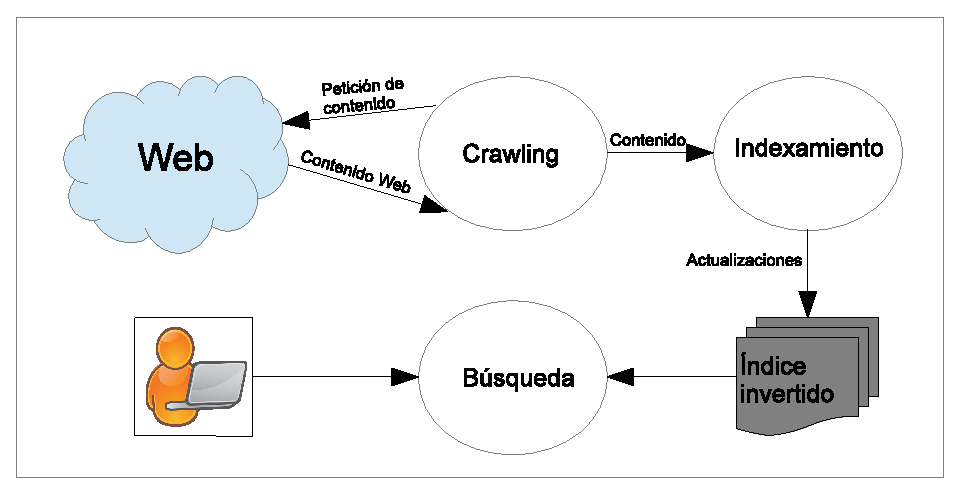
\includegraphics[scale=.75]{images/searchenginearchitecture.eps}
\caption{Arquitectura típica de un motor de búsqueda}
\label{fig:searchenginearchitecture}
\end{figure}

Dado el volúmen de datos involucrado en el procesamiento, se debe tener una estructura de datos que permita encontrar cuáles documentos contienen las palabras presentes en la búsqueda que llega al sistema. Todo esto dentro de un período de tiempo aceptable. El índice invertido \citep{Zobel:2006} es una estructura de datos que contiene un diccionario con todas las palabras que el proceso de \textit{crawling} ha encontrado, asociado a cada palabra se tiene una lista de todos los documentos en donde esta palabra aparece mencionada (conocida como lista invertida de un término). El motor de búsqueda construye esta estructura con el objetivo de acelerar el proceso de las búsquedas que llegan al sistema. El proceso de búsqueda es el encargado de recibir las transacciones de lectura, generar un \textit{ranking} de los documentos que contienen las palabras de la consulta y finalmente generar una respuesta. Las diversas formas de calcular la relevancia de un documento será explicado en secciones posteriores.

En un motor de búsqueda se pueden encontrar diversos servicios tales como (a) cálculo de los mejores documentos para una cierta consulta; (b) construcción de la página Web en la que se mostrará al usuario los resultados; (c) publicidad relacionada con las transacciones de lectura; (d) sugerencias en el momento que el usuario está escribiendo la consulta en el sistema; entre muchos otros servicios.

En los sistemas de recuperación de información como los motores de búsqueda, lo que se hace hoy en día es agrupar computadores para procesar una transacción y obtener la respuesta para ésta. Este conjunto de computadores recibe el nombre de \textit{cluster} \citep{Dean:2009}.

La diferencia entre un motor de búsqueda vertical y uno general, es que el primero se centra solo en un contenido específico de la Web \citep{Gil-Costa:2013}. El \textit{crawler} debe extraer contenido solo de aquellas páginas Web que están dentro del dominio permitido. Al ser un dominio acotado, los documentos a procesar serán menos y por lo tanto, la lista de los términos del índice invertido serán eventualmente de menor tamaño. Sin embargo, en un motor de búsqueda vertical las actualizaciones al índice invertido ocurren con mayor frecuencia.

\section{\'Indice invertido}
\label{marco:ii}
Es una estructura de datos que contiene todos los términos (palabras) encontrados por el \textit{crawler}. A cada uno de los términos está asociado una lista invertida de documentos (páginas Web) que contienen dicho término. Adicionalmente, se almacena información que permita realizar el \textit{ranking} de documentos para generar la respuesta a las consultas que llegan al sistema, por ejemplo, el número de veces que aparece el término en el documento.

Para construir un índice invertido \citep{Baeza-Yates:2011, Salton:2003} se debe procesar cada palabra que existe en un documento, registrando su posición y la cantidad de veces que éste se repite. Cuando se procesa el término con la información asociada correspondiente, se almacena en el índice invertido (ver Figura \ref{fig:invertedindex}).

\begin{figure}[!th]
\centering
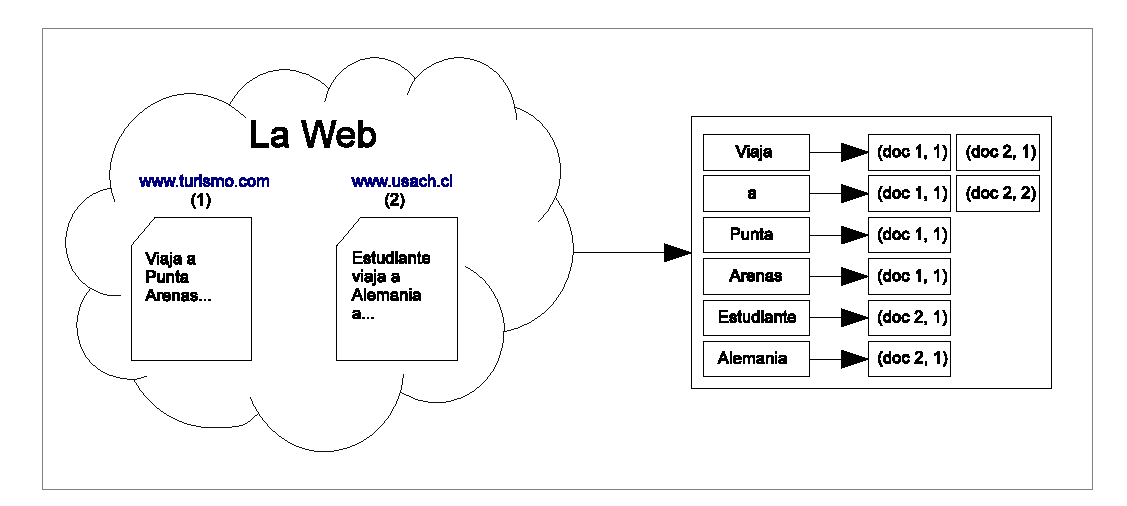
\includegraphics[scale=.75]{images/invertedindex.eps}
\caption{\'Indice invertido}
\label{fig:invertedindex}
\end{figure}

El tamaño del índice invertido crece rápido y eventualmente la memoria RAM se agota antes de procesar toda la colección de documentos. Cuando la memoria RAM se agota, se almacena en disco el índice parcial, se libera la memoria y se continúa con el proceso. Además, se debe hacer un \textit{merge} de los índices parciales uniéndo las listas invertidas de cada uno de los términos involucrados. Es por esto que se han desarrollado algunas técnicas de compresión con el objetivo de guardar de una manera más eficiente el índice invertido \citep{Arroyuelo:2013, Baeza-Yates:2011, Yan:2009}.

\section{Estrategias de evaluaci\'on de transacciones de lectura}
\label{marco:eeq}
Una de las tareas que un motor de búsqueda debe hacer para resolver una consulta es calcular el puntaje o \textit{score} para aquellos documentos relevantes en la consulta y así poder extraer los mejores $K$ documentos. Existen dos principales estrategias para recorrer las listas invertidas y calcular el puntaje de los documentos para una determinada consulta. Estas son (a) \textit{term-at-a-time} \citep{Buckley:1985, Turtle:1995} y (b) \textit{document-at-a-time} \citep{Broder:2003, Turtle:1995}.

\subsection{\textit{Term at a time}}
\label{marco:TAAT}
Abreviada TAAT, este tipo de estrategia procesa los términos de las consultas una a una y acumula el puntaje parcial de los documentos. Las listas invertidas asociadas a un término son procesadas secuencialmente, esto significa que todos los documentos presentes en la lista invertida del término $t_{i}$ obtienen un puntaje parcial antes de comenzar el procesamiento del término $t_{i+1}$. La secuencialidad en este caso es con respecto a los términos contenidos en la transacción de lectura.

\subsection{\textit{Document at a time}}
\label{marco:DAAT}
Abreviada DAAT, en este tipo de estrategias se evalúa la contribución de todos los términos de la transacción de lectura con respecto a un documento antes de evaluar el siguiente documento. Las listas invertidas de cada término de la consulta son procesadas en paralelo, de modo que el puntaje del documento $d_{j}$ se calcula considerando todos los términos de la transacción de lectura al mismo tiempo. Una vez que se obtiene el puntaje del documento $d_{j}$ para la consulta completa, se procede al procesamiento del documento $d_{j+1}$. Este tipo de estrategia posee dos grandes ventajas: (a) Requieren menor cantidad de memoria para su ejecución, ya que el puntaje parcial por documento no necesita ser guardado y (b) Explotan el paralismo de entrada y salida (I/O) más eficientemente procesando las listas invertidas en diferentes discos simultáneamente.

\section{Funciones de \textit{Ranking}}
\label{marco:ranking}
Los sistemas de recuperación de información como los motores de búsqueda deben ejecutar un proceso el cual asigna puntaje a documentos con respecto a una determinada transacción de lectura, este proceso se denomina \textit{ranking} \citep{Baeza-Yates:2011}. Como se puede ver en la Figura \ref{fig:ranking_process}, este proceso toma como entrada la representación de las consultas y documentos, y asigna un \textit{score} a un documento $d_{j}$ dada una consulta $q_{i}$.

Un motor de búsqueda guarda billones de documentos que están formados por términos o palabras, estos términos no todos poseen la misma utilidad para describir el contenido del documento. Determinar la importancia de una palabra en un documento no es tarea sencilla, para ello se asocia un peso positivo $w_{i,j}$ a cada término $t_{i}$ del documento $d_{j}$. De esta forma, para un término $t_{i}$ que no aparezca en el documento $d_{j}$ se tendrá $w_{i,j} = 0$. La asignación de pesos a los términos permite generar un \textit{ranking} numérico para cada documento en la colección.

\begin{figure}[!th]
\centering
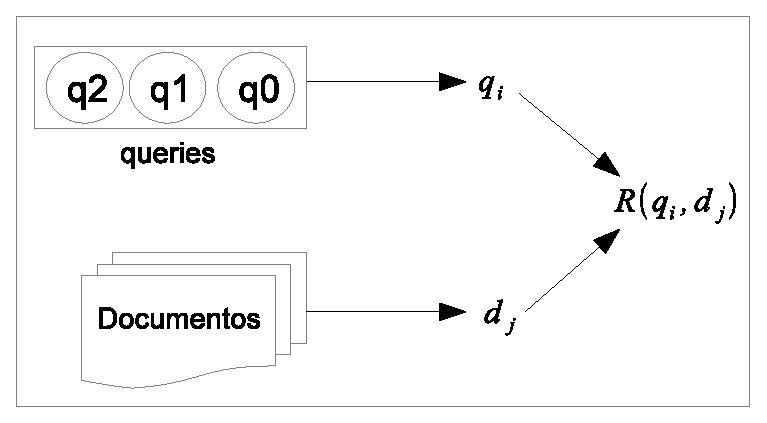
\includegraphics[scale=.75]{images/ranking_process.eps}
\caption{Proceso de \textit{scoring} de documento}
\label{fig:ranking_process}
\end{figure}

\subsection{TF-IDF}
\label{marco:tfi-df}
$Tf-idf$ (\textit{term frequency - inverse document frequency}) es un estadístico que tiene por objetivo reflejar cuán importante es una palabra para un documento en una colección o corpus %. Este estadístico se divide en dos partes, el primero corresponde a la frecuencia del término en un documento ($tf$) y que en su versión más sencilla se utiliza la frecuencia bruta del término $t$ en el documento $d$ ($f(t,d)$) dividido por la frecuencia de la palabra que más se repite en el documento $d$.  

\begin{equation}
\label{formula:tf}
tf(t,d) = \dfrac{f(t,d) }{ \max{f(w,d) : w \in d}}
\end{equation}

El segundo término corresponde a la frecuencia inversa de documento ($idf$) y se utiliza para observar si es que el término es común en el corpus. El $idf$ se obtiene calculando el logaritmo de la división entre el número total de documentos del corpus y el número de documentos que contienen el término.

\begin{equation}
\label{formula:idf}
idf(t,D) = log \frac{ |D| }{1 + |{d \in D : t \in d}|}
\end{equation}

De esta forma a partir de \eqref{formula:tf} y \eqref{formula:idf} se obtiene finalmente el $tf-idf$: 

\begin{equation}
\label{formula:tfi-df}
tf-idf(t,d,D) = tf(t,d) * idf(t,D)
\end{equation}

Notar en \eqref{formula:tfi-df} que el estadístico incrementa proporcionalmente al número de veces que la palabra aparece en el documento, sin embargo, es compensado por la frecuencia de la palabra en la colección completa de documentos o corpus. Esta compensación ayuda a controlar el hecho de que algunas palabras son generalmente más comunes que otras.


\subsection{BM25}
\label{marco:bm25}
Es una función de \textit{ranking} de documentos basada en los términos que aparecen en la consulta que llega al motor de búsqueda. \textit{BM25} pertenece a una amplia gama de funciones de puntuación y está basada en los modelos probabilísticos de recuperación de la información \citep{Baeza-Yates:2011}.

Dada una consulta $Q$ que contiene los términos $q_{1},...,q_{n}$, el \textit{ranking BM25} del documento D se calcula como: 

\begin{equation}
\label{formula:bm25}
score(D,Q) =  \displaystyle\sum_{i=1}^n IDF(q_{i}) * \frac{f(q_{i},D)*(k+1)}{f(q_{i},D)+k * (1 - b + b * \frac{|D|}{prom(docs)})}
\end{equation}

En donde: $f(q_{i}, D)$ es la frecuencia en que aparece el término $q_{i}$ en el documento D; $|D|$ es el número de palabras o términos en el documento D; $prom(docs)$ es la media de número de palabras de los documentos en el corpus; k y b son constantes que depende de las características del corpus en el que se está haciendo la búsqueda, por lo general se asignan los valores de $k = 2$ o $k = 1.2$ y $b = 0.75$; finalmente, $IDF(q_{i})$ es la frecuencia inversa de documento para el término $q_{i}$.


\section{Operaciones sobre listas invertidas}
\label{marco:osli}
Cuando una consulta llega al motor de búsqueda, cada término tiene asociado una lista con todos los documentos en los cuales aparece. El sistema debe decidir qué documentos se analizarán para obtener la respuesta y entregar al usuario una respuesta. A continuación se presenta los modos de operar las listas invertidas para una cierta transacción de lectura.

\subsection{\textit{OR}}
\label{marco:or}
Este operador toma las listas invertidas de cada uno de los términos de la transacción de lectura y ejecuta la disyunción entre ellas. El resultado de este operador es una lista invertida con todos los documentos que contengan al menos un término de la consulta. Finalmente, esta lista invertida se ocupará para obtener los mejores K documentos. Un simple ejemplo se muestra en la Figura \ref{fig:ORoperation}.

\begin{figure}[!th]
\centering
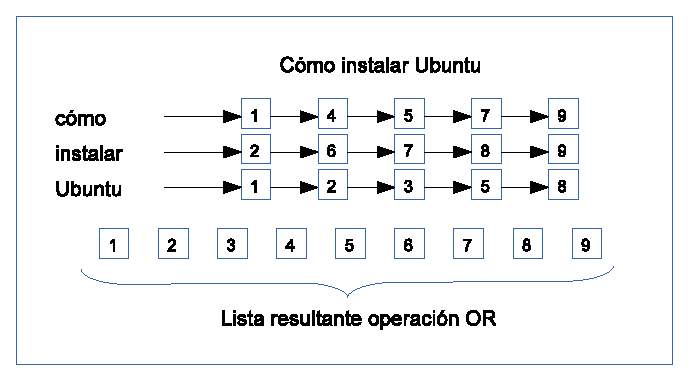
\includegraphics[scale=.75]{images/ORoperation.eps}
\caption{Operaci\'on OR}
\label{fig:ORoperation}
\end{figure}

\subsection{AND}
\label{marco:and}
Este operador ejecuta la conjunción entre las listas invertidas de los términos de una transacción de lectura. Se obtiene una lista invertida con los documentos que contengan todos los términos de la consulta. Se debe notar que aquí se obtiene una lista resultante de menor tamaño que la obtenida en el operador OR (Ver Figura \ref{fig:ANDoperation}).

\begin{figure}[!th]
\centering
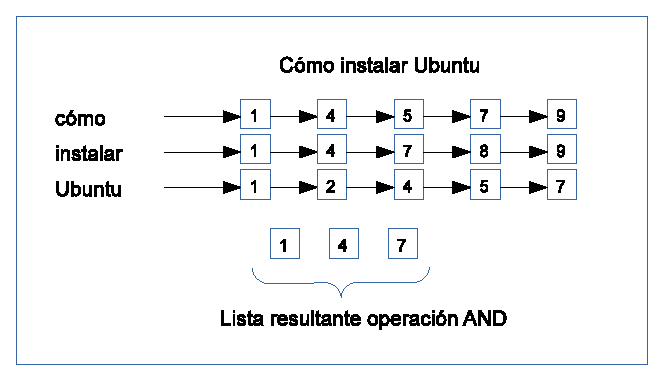
\includegraphics[scale=.75]{images/ANDoperation.eps}
\caption{Operaci\'on AND}
\label{fig:ANDoperation}
\end{figure}

\subsection{Wand}
\label{marco:wand}
Algoritmo de evaluación de transacciones de lectura para obtener eficientemente el conjunto de $K$ documentos que mejor satisfacen una consulta dada. WAND \citep{Broder:2003} es un proceso menos estricto que el método \textit{AND} y está basado en dos niveles. Dentro del proceso de evaluación de una transacción de lectura, uno de los procesos más costoso en términos de tiempo es el de \textit{scoring}, que consiste en entregarle a cada uno de los documentos analizados un puntaje que representa la relevancia del documento para una transacción de lectura dada, esto se denomina evaluación completa o cálculo del puntaje exacto del documento. El objetivo de WAND es minimizar la cantidad de evaluaciones completas de los documentos ejecutando un proceso de dos niveles. En el primer nivel se intenta omitir rápidamente grandes porciones de las listas invertida, lo que se traduce en ignorar el cálculo del puntaje exacto de grandes cantidades de documentos, esto porque en motores de búsqueda a gran escala, este un proceso que requiere de mucho tiempo para llevarse a cabo y depende de factores como la cantidad de ocurrencia del término dentro del documento, el tamaño del documento, entre otros. A este tipo de técnicas que intenta omitir partes de lista invertida se les conoce como técnica de poda dinámica \citep{Broder:2003, Persin:1994, Turtle:1995}. 

Para llevar a cabo el algoritmo WAND y así reducir el número de documentos completamente evaluados durante el proceso de \textit{ranking} de documentos, se necesita calcular los valores estáticos de límite superior (\textit{upper-bounds}), en donde para cada uno de los términos del índice invertido, se toma la lista invertida correspondiente y se extrae el puntaje máximo de contribución de algún documento con respecto al término. El cálculo de los \textit{upper bounds} se lleva a cabo cuando se construye el índice invertido y en donde a cada término del índice se asocia el puntaje máximo que existe en la lista invertida. 

WAND usa un índice invertido ordenado por los identificadores de documentos. En el primer nivel se itera sobre los documentos del índice invertido de cada término y se identifican los potenciales candidatos usando una evaluación aproximada. En el segundo nivel, aquellos documentos candidatos son completamente evaluados y su puntaje exacto es calculado. De esta forma se obtiene el conjunto final de documentos. Se utiliza un heap como estructura de datos para almacenar el conjunto de los mejores $K$ documentos, en donde el elemento superior corresponde al documento con menor puntaje y es el que se utilizará como umbral (\textit{threshold}) para decidir si los siguientes documentos deben ser completamente evaluados o no.

En la Figura \ref{fig:proceso_wand} se puede ver un ejemplo sencillo de cómo el algoritmo Wand trabaja en la resolución de una transacción de lectura de tres términos: 'casa', 'perro' y 'gato'. Como la consulta está compuesta por tres términos, existen tres punteros que recorren cada una de las listas invertidas (notar que cada puntero recorre una lista invertida diferente). Lo primero que se hace es ordenar las listas invertidas de acuerdo a los identificadores de documentos que se están apuntando, razón por la cual en la Figura \ref{fig:proceso_wand} la lista invertida de 'casa' (puntero referenciando al documento con identificador 125), aparece primero que la lista invertida de 'perro' (puntero haciendo referencia al documento con identificador 503). Luego se suma los \textit{uppers bounds} de los términos en orden hasta que se obtiene un valor mayor o igual al \textit{threshold}. De esta manera el término 'perro' es escogido como término pivote ($2.0 + 4.4 \geq 5.7$) y el actual documento al cual se está apuntando es escogido como documento pivote (documento con identificador 503). Si las dos primeras listas invertidas no contienen el documento 503 entonces se procede a seleccionar el siguiente pivote, en otro caso se calcula el puntaje completo del documento. Finalmente, si el puntaje es mayor o igual al \textit{threshold}, se actualiza el \textit{heap} eliminando el elemento superior y se añade el nuevo documento. 
Este algoritmo es repetido hasta que no hayan más documentos a procesar o hasta que no exista un documento que supere el actual \textit{threshold}. De esta manera se evita procesar las listas completas \citep{Blanco:2010}.

\begin{figure}[!th]
\centering
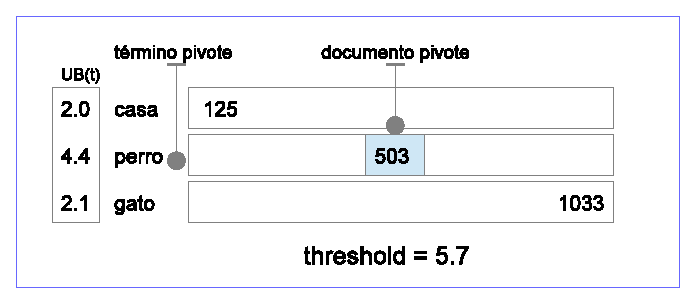
\includegraphics[scale=.75]{images/proceso_wand.eps}
\caption{Ejemplo de ejecución de algoritmo Wand}
\label{fig:proceso_wand}
\end{figure}

\subsection{Block Max Wand}
\label{marco:bmw}
Como se explicó en la sección anterior, la diferencia entre un método exhaustivo de evaluación de documentos y el método Wand, es que este último es una técnica DAAT de poda dinámica \citep{Moffat:1996} en la que se intenta omitir la mayor cantidad de evaluaciones de documentos haciendo uso de una estrategia de movimientos de punteros pivotes.
Bajo la premisa que Wand tradicional es limitado por el hecho que usa los máximos puntajes de las listas invertidas (\textit{Upper bounds}) para podar, puesto que estos pueden ser mucho más grandes que el promedio de puntaje en ellas, se propone un método llamado \textit{Block-Max-Wand} (BMW) \citep{Ding:2011}. Este método utiliza una estructura de datos llamada índice \textit{Block-Max}, en donde el índice invertido estará particionado en bloques y para cada bloque se almacena la máxima contribución de algún documento dentro del bloque. En otras palabras, se tendrán tantos \textit{upper bounds} locales como bloques existan en la lista invertida.

Este método utiliza una variación del algoritmo Wand tradicional para que trabaje correctamente con la nueva estructura \textit{Block-Max-Wand}. Remplazar el uso de los \textit{upper bounds} de cada bloque por el \textit{upper bound} global no garantiza la correctitud del algoritmo. En la Figura \ref{fig:bmw} se muestra un ejemplo de por qué mirar solo los \textit{upper bounds} locales no garantiza obtener los resultados correctos, aquí no se puede concluir que el documento 4868 es el documento más pequeño que puede estar dentro del conjunto \textit{top-K}, ya que $2.5 + 2.0 + 3.5 \geq 7.0$ (conclusión que sí es válida utilizando Wand tradicional y \textit{upper bounds} globales), porque es posible que el bloque siguiente al bloque del docID 275 (en la primera lista), tenga un \textit{upper bound} local mayor. Por lo tanto, aplicar solo las máximas contribuciones por bloque no permite al algoritmo omitir documentos de forma segura.  

\begin{figure}[!th]
\centering
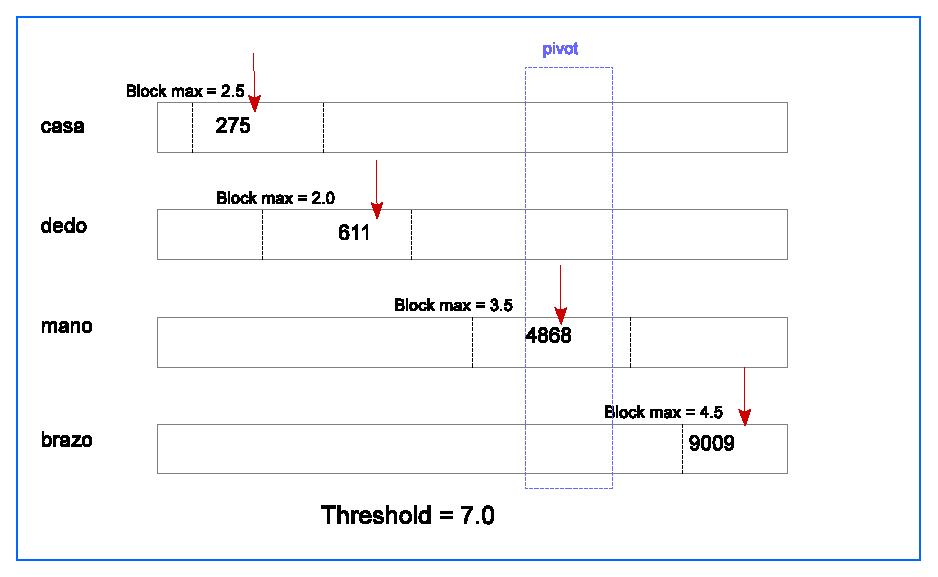
\includegraphics[scale=.75]{images/block-max-wand.eps}
\caption{Ejemplo del proceso \textit{Block-Max-Wand}}
\label{fig:bmw}
\end{figure}

\section{Predicción de tiempo de respuestas de transacciones de lecturas}
\label{marco:prediccion}
El rendimiento (\textit{performance}) de una consulta puede medirse de dos formas: Efectividad y eficiencia. La efectividad tiene relación con la calidad de los documentos extraídos para una cierta consulta y la eficiencia corresponde al tiempo que conlleva procesarla. El tiempo que le toma al sistema en resolver una consulta puede variar considerablemente. Con el objetivo de retornar los resultados al usuario dentro de una cota superior de tiempo, aquellas consultas que toman una mayor cantidad de tiempo en ser procesadas se requiere una mayor cantidad de procesadores para resolverla, de esta forma podemos asegurar esta cota de tiempo. El tener un buen predictor de la eficiencia de una transacción de lectura es muy útil, por ejemplo, si pensamos en un sistema con réplicas, podemos planificar la consulta en el servidor que se desocupará más pronto. 

Existen estudios en los cuales el rendimiento es inferido usando \textit{clarity score} \citep{Cronen-Townsend:2002}, que es una forma para evaluar la pérdida de ambigüedad de una transacción con respecto a la colección. En \citep{He:2004} se propone un conjunto de predictores para el rendimiento de cada consulta. Técnicas de aprendizaje de máquina también han sido estudiadas para predecir el rendimiento de transacciones de lectura \citep{Si:2002}. Todos los estudios mencionados anteriormente se han centrado en la efectividad para ser predicciones de rendimento de transacciones de lectura. La eficiencia de una transacción de lectura también ha sido objeto de estudio, identificando las principales razones que tienen impacto sobre el tiempo de respuesta y evaluando estos factores para predecir el comportamiento de futuras consultas \citep{Tonellotto:2011}. En \citep{Macdonald:2012} se propone un método de predicción de tiempo de respuesta para consultas basado en datos estadísticos disponibles en las respectivas listas invertidas de los términos. Finalmente, en \citep{Jeon:2014} además de utilizar estadísticos disponibles en las listas invertidas de los términos, se agregan estadísticos propios de las consultas para la creación de un predictor. 

\section{Scheduling en motores de búsqueda}
\label{marco:scheduling}
Los motores de búsqueda no solo se preocupan de la calidad de los resultados de las búsquedas (efectividad), sino que también de la velocidad con la que los resultados son obtenidos (eficiencia). Existen varias estrategias para mejorar la velocidad en la obtención de los resultados, una de ellas muy utilizada es el \textit{caching}. Consiste en guardar en memoria de acceso rápido (memoria caché) datos temporales, que luego pueden ser sobrescritos. Una opción es hacer \textit{caching} de los resultados de las búsquedas, de esta forma cuando una consulta es encontrada en caché el motor de búsqueda puede generar la respuesta rápidamente, reduciendo considerablementelos tiempos de calculos. Otra opción es, guardar en caché la intersección de las listas invertidas de pares comunes de términos que llegan al motor de búsqueda. Por ejemplo, si llega al sistema una consulta con los términos ('casa', 'árbol', 'perro'), se puede guardar en caché la intersección de las listas de 'casa' y 'árbol', para luego reutilizar esta información en otras consultas que lleguen en el futuro. Para ver más técnicas de \textit{caching} y ver el detalle de las técnicas mencionadas, ver \citep{Buttcher:2010}. 

Otra estrategia para acelerar el proceso de resolución de transacciones de lectura que llegan al sistema es el uso de algoritmos de planificación (scheduling). Un algoritmo de \textit{scheduling} es el proceso en el cual se cambia el orden en que llegan las consultas al motor de búsqueda con el objetivo de mejorar la eficiencia. 

Existen dos clases de algoritmos de \textit{scheduling}: estáticos y dinámicos. Los estáticos son aquellos en que se conoce el conjunto completo de tareas y las características de cada una de ellas, como por ejemplo, el tiempo de procesamiento. Los algoritmos de \textit{scheduling} dinámicos son aquellos en que no se conoce las tareas que llegarán en el futuro, también se desconoce el momento en que éstas llegarán. La filosofía de los algoritmos de \textit{scheduling} dinámicos es ajustarse a los cambios que pueden haber en el sistema.

En el contexto del presente trabajo de tesis, el objetivo de hacer \textit{scheduling} es minimizar el tiempo en que las consultas son procesadas por un motor de búsqueda. Los motores de búsqueda como \textit{Google}\footnote{http://www.google.com} o \textit{Yahoo!}\footnote{http://www.yahoo.com} trabajan en un contexto \textit{online}. Esto significa que cuando las consultas llegan al sistema (una a una), éste está obligado a tomar una decisión para planificarla sin saber cuáles transacciones de lectura llegarán en un momento posterior. A esto se le conoce como algoritmo de \textit{scheduling online} \citep{Albers:2003, Borodin:1998}.

Los sistemas de recuperación de información a gran escala despliegan una arquitectura distribuída \citep{Dean:2009}, en donde el índice invertido está particionado \citep{Barroso:2003} a lo largo de servidores (\textit{shard servers}), los cuales están encargados de procesar las transacciones de lectura que llegan al sistema. Es fácil notar que resolver una consulta con varios \textit{shard servers} mejoraría la eficiencia. Ahora bien, para asegurar un alto rendimiento (\textit{throughput}) del sistema, cada uno de los \textit{shard servers} poseen réplicas, de esta forma, más consultas pueden ser procesadas en paralelo en copias idénticas del mismo \textit{shard server}. Esto implica que el tiempo de espera de las transacciones de lectura que vienen llegando al sistema se reduce. 

En un sistema con arquitectura como el de la Figura \ref{fig:sistemaIR}, una transacción de lectura puede ser procesada por varios \textit{shard servers}, el \textit{broker} debe escoger la réplica más apropiada para procesar la parte de la consulta asignada al \textit{shard server}, con el objetivo de reducir el tiempo de espera de ésta. El \textit{broker} podría seleccionar el \textit{shard server} con el menor número de consultas en la cola, sin embargo, este no es un parámetro adecuado, ya que el tiempo de respuesta de las transacciones de lectura puede variar considerablemente, especialmente si se usa poda dinámica \citep{Broder:2003, Moffat:1996}. 

\begin{figure}[tp]
\centering
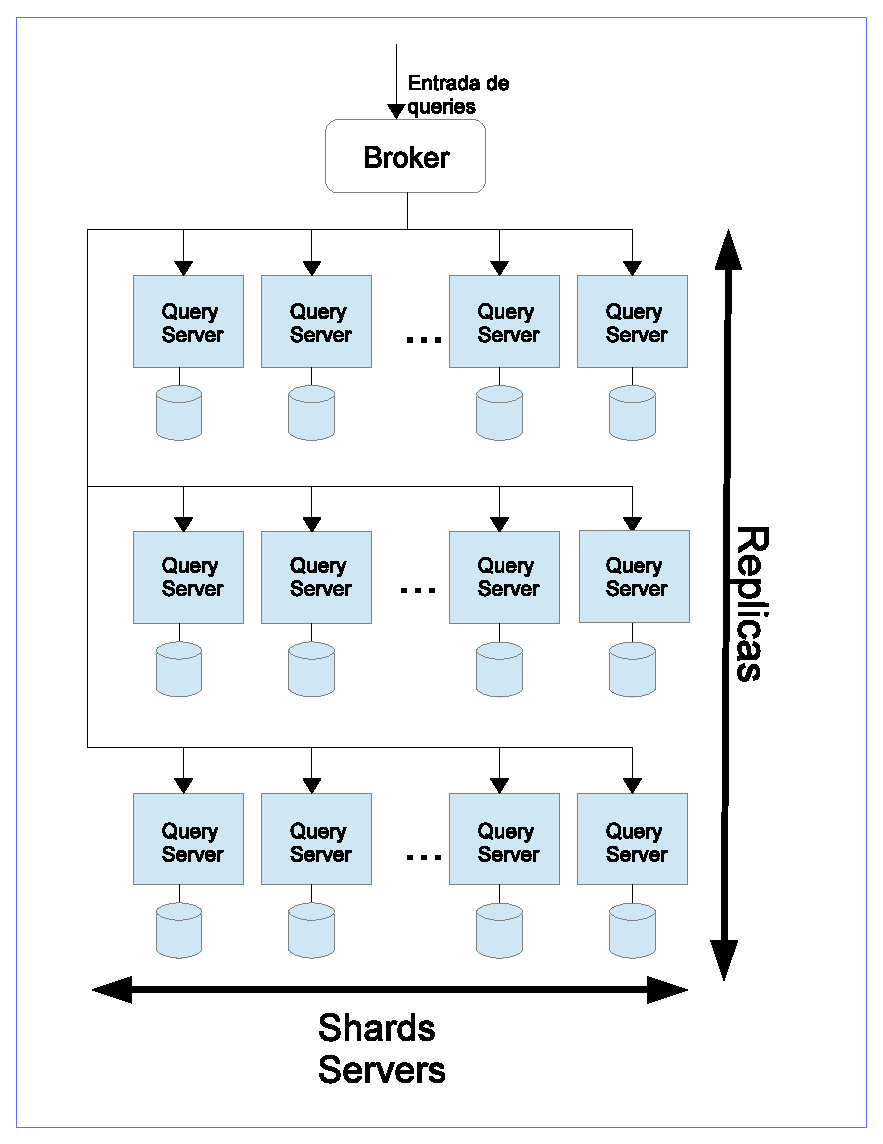
\includegraphics[scale=.75]{images/sistemaIR.eps}
\caption{Arquitectura de un sistema de recuperación de la información con réplicas}
\label{fig:sistemaIR}
\end{figure}

\subsection{Trabajo relacionado}
\label{marco:tr}
El estudio \citep{Broccolo:2013} analiza métodos de \textit{dropping} y \textit{stopping} para el procesamiento de consultas bajo altas carga de trabajo en un sistema distribuído donde existen múltiples servidores en el que cada uno resuelve una parte de la consulta para luego enviar las consultas al \textit{broker} y éste hace el \textit{merge} de los resultados de acuerdo al \textit{score} de los documentos. Se define un tiempo \textit{T}, en el que la suma de el tiempo de espera de la consulta para ser procesada ($t_{w}$) y el tiempo de procesamiento de la misma ($t_{p}$) deben ser menor a \textit{T}. Si es que se sobrepasa este tiempo, se tienen dos opciones (1) la consulta es desechada y se envía al \textit{broker} una lista vacía, (2) se detiene el procesamiento de la transacción de lectura y se envía los resultados parciales hasta el momento. Finalmente se propone un método basado en la predicción de tiempo de respuesta ($\hat{pt}(q)$) de una consulta \citep{Macdonald:2012} de modo que si se cumple $ \hat{pt}(q) \leq T - wt(q) $, entonces la consuta es desechada antes de comenzar a procesarse y se toma la siguiente desde la cola de espera. Notar que en estos métodos existe una pérdida de efectividad, puesto que eventualmente los servidores muchas veces no enviarán sus mejores documentos al \textit{broker}, esto implica que el \textit{broker} responderá al usuario un conjunto de K documento que no necesariamente son los mejores dentro del corpus completo.

En \citep{Freire:2012} se estudia el impacto que tiene la técnica de predicción de tiempos de respuestas para consultas, \citep{Tonellotto:2011} en sistemas de recuperación de la información con réplicas. En este estudio, se llega a la conclusión que usando una buena predicción, se puede reducir el tiempo que la consulta tiene que esperar para ser procesada ($t_{w}$), y también se puede reducir el tiempo total requerido para procesar el conjunto (\textit{log}) completo de transacciones de lectura (\textit{completion time}). En \citep{Freire:2013}, se propone un modelo híbrido de \textit{scheduling} de consultas a través de réplicas, en el que cuando el sistema se encuentre bajo altas cargas de trabajo, se utilice política de \textit{scheduling} basada en la predicción de tiempo de respuesta de las consultas \citep{Macdonald:2012} y cuando el sistema se encuentre con una baja carga de trabajo, se utilice una politica de \textit{scheduling} sencilla y de menor costo como \textit{Round Robin}.
\chapter{Wand \textit{multi-threaded}}
\label{cap:wand}
Dado que el método Wand \citep{Broder:2003} consiste en el método del estado del arte ocupado hoy en día por los motores de búsqueda para obtener eficientemente los mejores K documentos, en este trabajo se utiliza un sistema que trabaja con este método. Este algoritmo usa un \textit{ranking} basado en una evaluación de dos niveles. En el primer nivel, usa una cota superior (\textit{upper bound}) al puntaje de cada documento para intentar descartarlos eficientemente. En el segundo nivel se computa el puntaje real de los documentos que pasa el primer nivel. Se utiliza una estructura de datos llamada \textit{heap} que va guardando el conjunto de los mejores $K$ documentos hasta un determinado instante. El menor puntaje de este conjunto es usado como umbral (\textit{threshold}) para las evaluaciones del primer nivel, de esta forma se descarta rápidamente documentos que no pueden ser parte del conjunto final de los \textit{top-K} documentos. Esto permite un eficiente y a la vez seguro proceso de descarte que asegura que en el resultado final se encontrará el conjunto correcto y no se perderán documentos relevantes.

Existe una variación al método Wand tradicional que intenta hacer una poda más agresiva, en otras palabras, lo que se intenta es tratar de omitir una mayor cantidad de documentos a la hora de resolver una transacción de lectura. Este método llamado Block Max Wand requiere que cada una de las listas invertidas este particionada en bloques (generalmente 64 o 128 bloques), en donde se tiene un upper bound por cada bloque. La lógica es la misma que en el método original y en la primera fase también se ocupa el máximo puntaje por lista para descartar documento, sin embargo, ahora existe una tercera fase en donde se utiliza el upper bound por bloques. De esta forma se intenta omitir una mayor cantidad de documentos. Más detalle de estos métodos se pueden encontrar en las secciones \ref{marco:wand} y \ref{marco:bmw}.

Wand y Block Max Wand son métodos lógicamente parecidos en el sentido que trabajan con \textit{upper bounds} para poder descartar documentos, es por esto que el diseño de la implementación es como lo muestra la Figura \ref{fig:diagramawand}; aquí se puede apreciar dos tipos de Wand: WandScorer y WandMaxBlock. WandScorer implementa el método tradicional utilizando el método \textit{next}, que retornará algún documento que merezca estar en el conjunto \textit{top-K} en ese momento. Por su parte, WandMaxBlock además de utilizar la función \textit{$next()$}, usa la función \textit{$nextShallow()$}, que moverá el puntero del documento actual de la lista a la posición inicial del bloque en donde debería encontrarse el documento que se le entrega como parámetro. 
La ventaja de este diseño es que ambas opciones son flexibles a utilizar cualquier función de \textit{ranking} que se desee, en el diagrama se observa que se utilizará BM25.

\begin{figure}[!th]
\centering
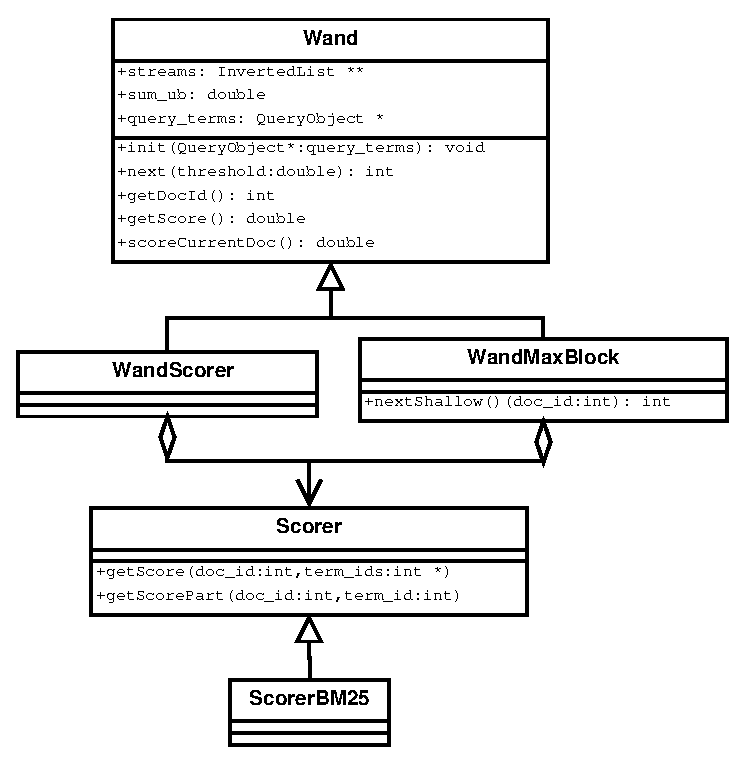
\includegraphics[scale=.75]{images/WAND.eps}
\caption{Diseño de clases para Wand y Block Max Wand.}
\label{fig:diagramawand}
\end{figure}

Existen dos formas de implementar Wand. Una de ellas es usando \textit{heaps} locales (LH), es decir, un \textit{heap} por hilo de ejecución y el otro es usando \textit{heaps} compartidos (SH). En el estudio \citep{Rojas:2013} se muestran indicios que el esquema SH es generalmente más eficiente, logrando rápidamente un óptimo valor para el \textit{threshold}. El esquema SH posee las siguientes ventajas: (1) Se puede reducir el número de cálculos de puntajes completos y (2) se ejecutan pocas operaciones de actualización del \textit{heap} (reduciendo el número de \textit{locks} que se hace a la estructura de dato). 
A continuación se muestra las dos formas en que se implementó Wand y también la implementación de Block Max Wand.


\section{Wand con \textit{heaps} locales}
\label{scheduling:wlh}
En el esquema LH, cada hebra procesa una parte del índice invertido mientras mantiene un \textit{heap} local con los mejores $K$ documentos. Al finalizar este proceso, los resultados se unen en un solo conjunto final global. Los resultados en \citep{Rojas:2013} muestran que el esquema LH es más eficiente para aquellas transacciones que toman poco tiempo en ser resueltas. En la Figura \ref{fig:wand-heap-local} se muestra el esquema de ejecución para \textit{heaps} locales explicado anteriormente. 

\begin{figure}[!ht]
\centering
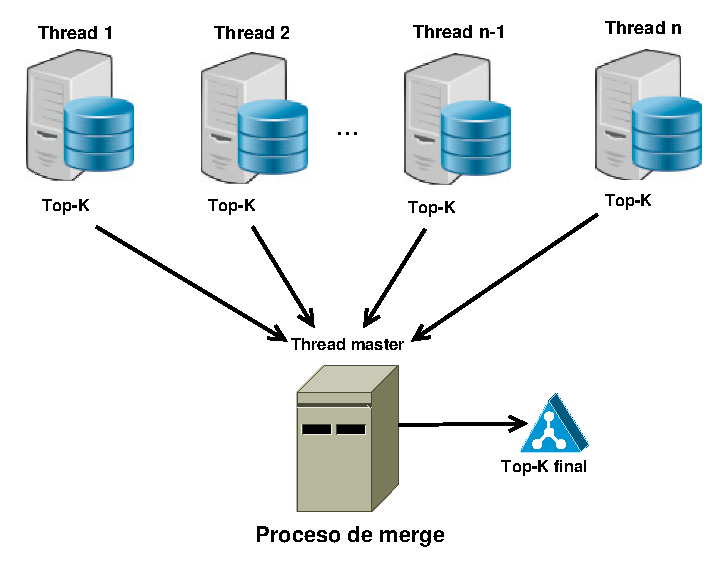
\includegraphics[scale=.75]{images/wand_heaps_locales.eps}
\caption{Esquema de ejecución de algoritmo WAND con \textit{heaps} locales.}
\label{fig:wand-heap-local}
\end{figure}

El diseño aplicado para implementar el esquema LH se puede ver en la Figura \ref{fig:TopKMultiThreadWandOperatorLocal}. La clase principal es la TopKMultiThreadWandOperatorLocal, que es la encargada de controlar el paralelismo en la resolución de las transacciones. Para explicar de mejor manera cada una de las clases involucradas en la implementación, se presenta el siguiente diccionario de datos.

\begin{figure}[!ht]
\centering
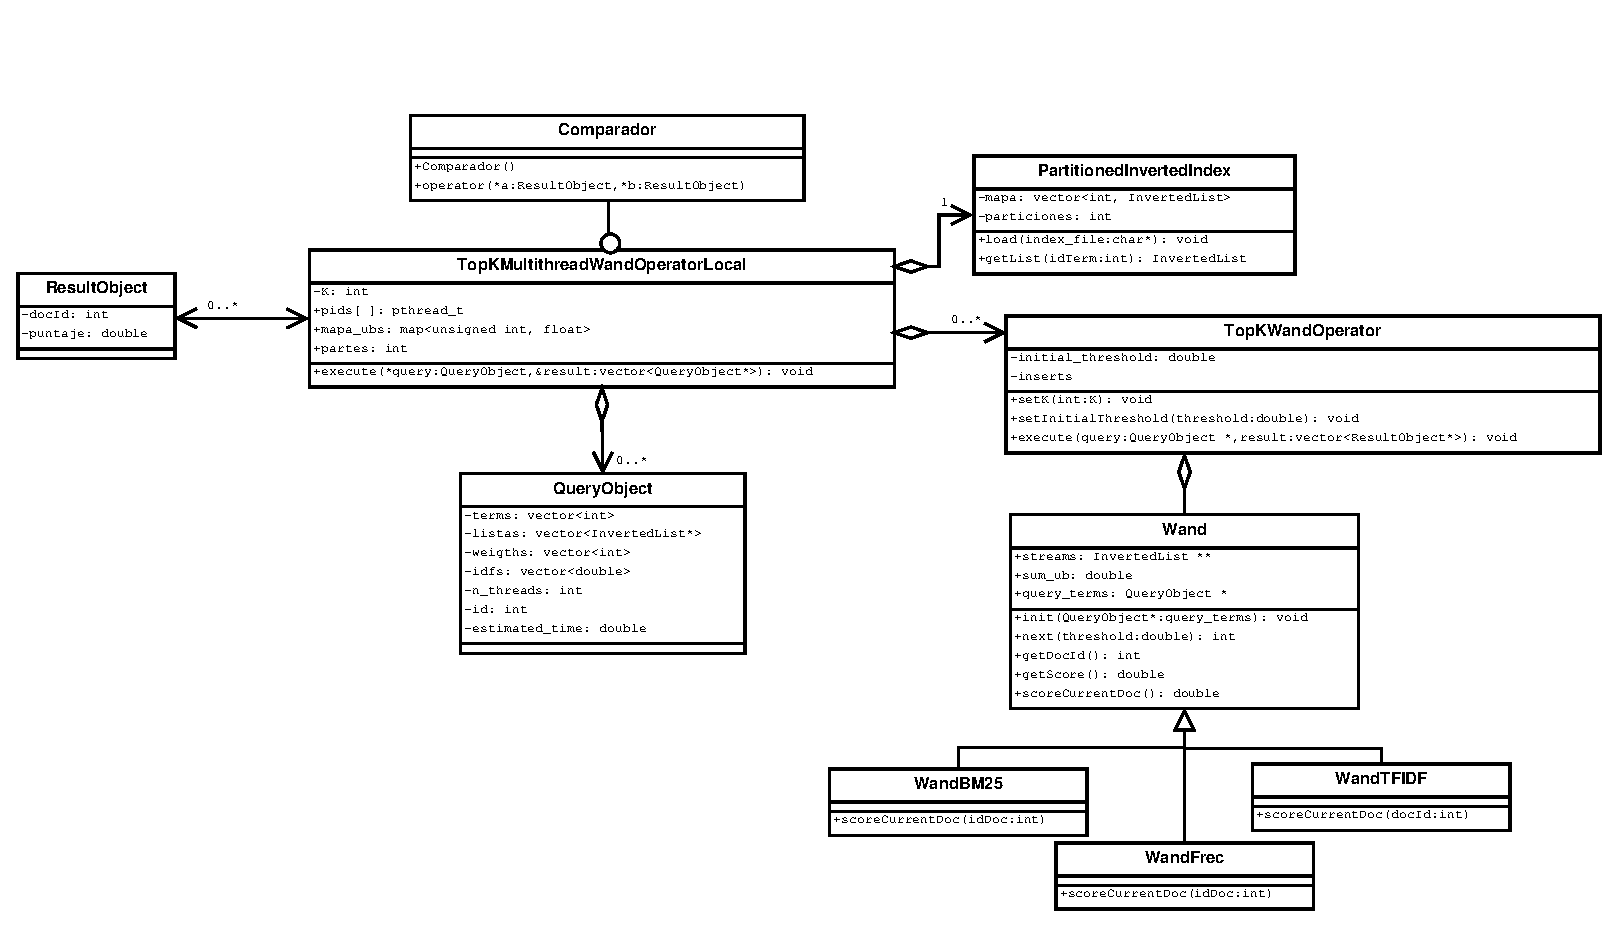
\includegraphics[scale=.75]{images/TopKMultiThreadWandOperatorLocal.eps}
\caption{Diagrama de clases para el esquema LH.}
\label{fig:TopKMultiThreadWandOperatorLocal}
\end{figure}

\begin{list}{}{}
	\item \textbf{TopKMultiThreadWandOperatorLocal}. Clase encargada de devolver los mejores $K$ documentos para una consulta dada. Si es que la consulta debe ser resuelta en forma paralela, esta clase además debe controlar el paralelismo que se produce en la resolución de ésta, inicializando las variables correspondientes para lanzar los hilos de ejecución y luego escogiendo los mejores documentos desde todos los \textit{heaps} creados por los diferentes hilos de ejecución (proceso de \textit{merge}). En esta clase se define un mapa que asocia cada término del índice invertido con el puntaje del mejor documento en esa lista invertida (upper bound de la lista invertida) y además se define cuántos documentos se van a retornar al final del proceso (atributo K). El método \textit{execute} inicializa las variables locales para las diferentes hebras, posteriormente hace el llamado al método \emph{thread-execute} (en el cual se llevará a cabo la resolución de la transacción de lectura en forma paralela), finalmente se toman los resultados parciales de cada uno de los hilos de ejecución y se ejecuta el proceso que mezcla los resultados, retornando solo los mejores $K$ documentos. 
	
	\item \textbf{PartitionedInvertedIndex}. Clase que tiene la tarea de almacenar el índice invertido y extraer desde aquí las listas invertidas de documentos para cada uno de los términos de las transacciones de lectura. El almacenamiento del índice se lleva a cabo mediante un mapa, en donde cada término tiene asociado su lista invertida correspondiente y para la extracción de estas listas se usa el método getList.
	
	\item \textbf{TopKWandOperator}.  Cada hilo tendrá su propio objeto TopKWandOperator encargado de obtener los mejores $K$ documentos. El cálculo de este conjunto se realiza en el método \textit{execute} con la ayuda de un objeto de tipo Wand asociado.
	
	\item \textbf{Wand}. Clase que controla la lógica del algoritmo wand. Lleva a cabo el proceso de inserción de documentos en el \textit{heap} y todo lo que esto conlleva. Existen diferentes tipos de objetos Wand que se pueden utilizar, entre ellos están WandBM25, WandFrec y WandTFIDF, donde la única diferencia entre ellos es el método con que se calcula el puntaje de cada documento. Por ejemplo, WandBM25 utiliza BM25 y WandTFIDF utiliza tf-idf. 
	
	\item \textbf{ResultObject}. Clase que se utiliza para guardar los mejores $K$ documentos.
	
	\item \textbf{QueryObject}. Clase que representa una transacción de lectura. Está formada por términos y sus respectivas listas invertidas, la cantidad de hebras con las cuales se resolverá dicha transacción y el tiempo estimado de procesamiento (este tiempo se predice al momento de resolver la consulta).

\end{list}


\section{Wand con \textit{heap} compartido}
\label{scheduling:whc}
En el esquema SH cada hebra procesa una parte del índice. Sin embargo, ahora un solo \textit{heap} es creado y accedido por todos los hilos de ejecución. En este caso no se requiere de mezclar los resultados y el proceso de descarte tiende a ser más eficiente porque los documentos con mayor puntaje tienden a estar en el \textit{heap}. El acceso al \textit{heap} debe ser controlado por un \textit{lock} o algún método similar que garantice el acceso exclusivo de los hilos al \textit{heap}. Este esquema es más eficiente que el LH en consultas que toman mayor tiempo en ser resueltas.

El diseño implementado para este esquema posee como clase principal a TopKMultiThreadWandOperatorLocks y difiere del modelo implementado para el esquema LH en el sentido que ahora se debe controlar el acceso concurrente a los datos compartidos como el \textit{heap} y el \textit{threshold}. A continuación se presenta el diccionario de datos del esquema SH mostrado en la Figura \ref{fig:TopKMultiThreadWandOperatorLocks}.

\begin{figure}[!ht]
\centering
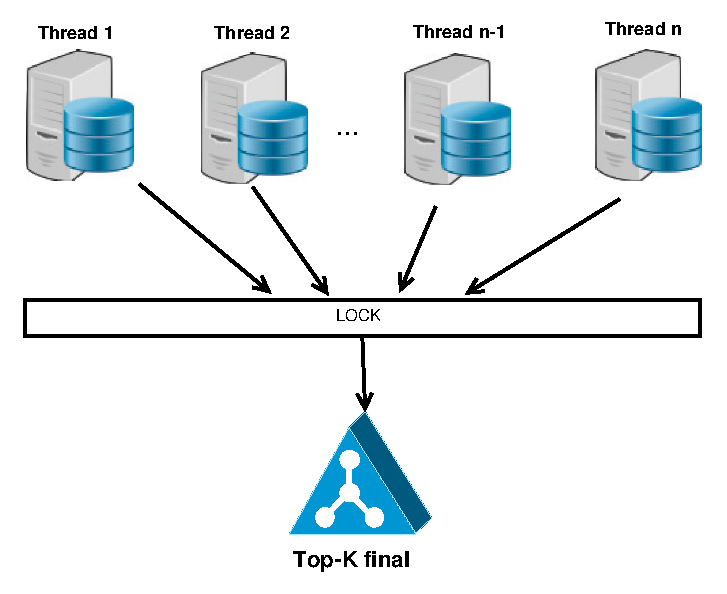
\includegraphics[scale=.75]{images/wand_heaps_compartido.eps}
\caption{Esquema de ejecución de algoritmo WAND con \textit{heap} compartido.}
\label{fig:wand-heap-compartido}
\end{figure}

\begin{list}{}{}
	\item \textbf{TopKMultiThreadWandOperatorLocks}. Clase encargada de inicializar las variables compartidas y de lanzar los hilos de ejecución requeridos para procesar la transacción de lectura.
	
	\item \textbf{WandThreadData}. Clase anidada a TopKMultiThreadWandOperatorLocks que contendrá todas las variables compartidas para el procesamiento de las consultas. Dentro de los atributos más importantes destaca el mutex utilizado para controlar el acceso al \textit{heap} compartido y además al \textit{threshold} (en este esquema es un \textit{threshold} global y compartido por todas las hebras).
	
	\item \textbf{Wand}. Al igual que en el esquema anterior, esta clase se encarga de llevar a cabo el proceso de inserción de documentos en el \textit{heap} y de las actualizaciones del \textit{threshold}. El método \textit{scoreCurrentDoc} es el encargado de entregarle un puntaje a cada documento y dependerá de qué tipo de Wand se este utilizando (BM25, WandFrec, WandTFIDF). 

	\item \textbf{PartitionedInvertedIndex}. Clase encargada de almacenar el índice invertido. Posee un método llamado getList que recibe como parámetro el identificador de un documento y retorna la lista invertida asociada. 

\end{list}

\begin{figure}[!ht]
\centering
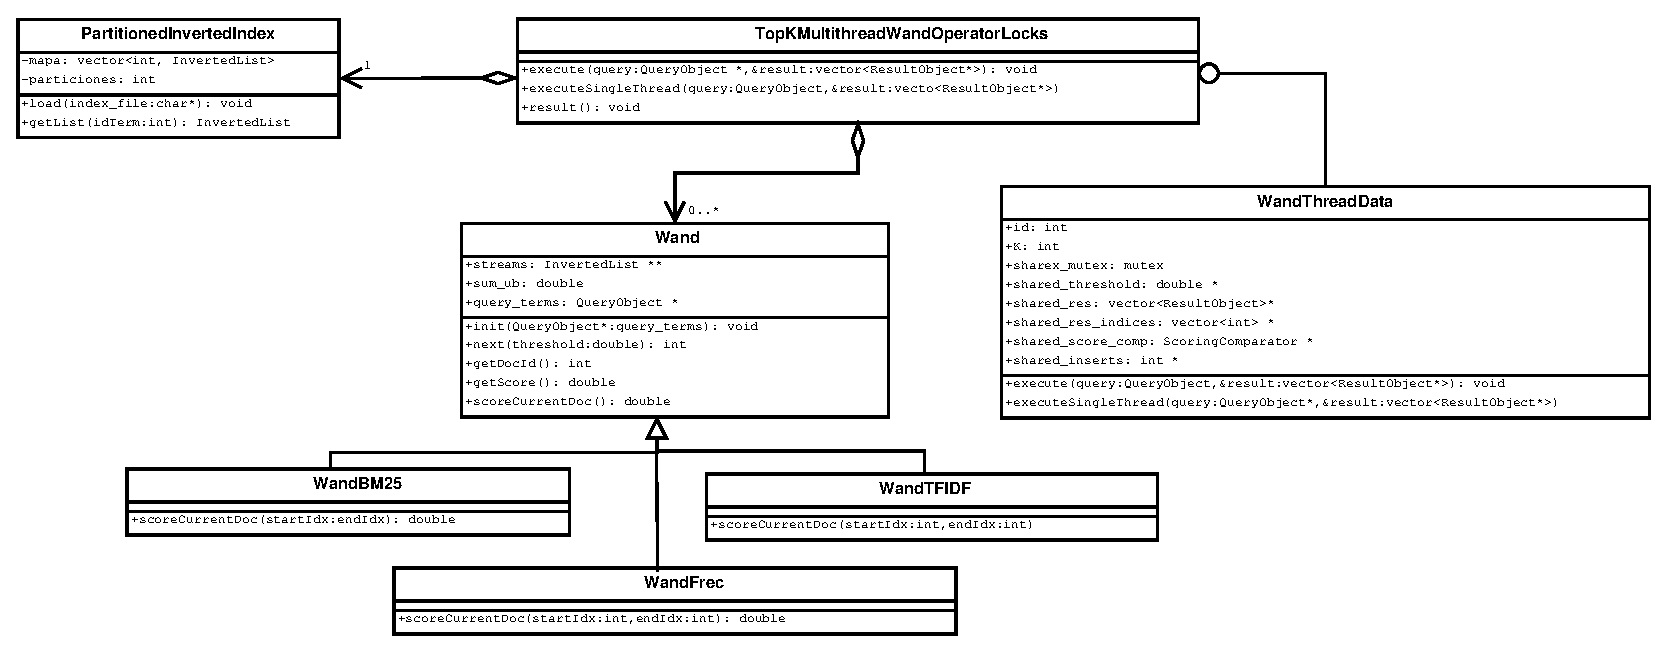
\includegraphics[scale=.75]{images/TopKMultiThreadWandOperatorLocks.eps}
\caption{Diagrama de clases para el esquema SH.}
\label{fig:TopKMultiThreadWandOperatorLocks}
\end{figure}

\section{Block max wand}
Recordar que en el método de Wand para descartar documentos y encontrar un documento que potencialmente podría estar en el conjunto \textit{top-K}, utiliza los \textit{upper bounds} globales de cada lista, es decir, la máxima contribución (puntaje o \textit{score}) de algún documento de la lista invertida. Además, Wand tradicional es una estrategia DAAT, por lo que por cada lista invertida ocupa un puntero al documento actual que se desea evaluar; también usa un método que recibe como entrada un identificador del documento $docID$ y una lista invertida $L$, y retorna el primer $docID'$ que sea mayor o igual al documento $docID$. A esto se le conoce como movimiento de puntero profundo (\textit{deep pointer movement}) debido a que generalmente implica una descompresión del bloque en el que se encuentra el documento.

Sin embargo, como se dijo anteriormente en \ref{marco:bmw}, usando solo las máximas contribuciones por cada bloque no hará que el método funcione correctamente, puesto que hará que eventualmente se pierdan documentos que podrían estar en el conjunto final de los mejores $K$ documentos. Como ahora se tiene las máximas contribuciones por cada bloque, BMW utiliza otra función la cual recibe como parámetro un identificador de documento $docID$ y una lista invertida. Lo que se hace es mover el puntero actual al correspondiente bloque donde eventualmente se debería encontrar el documento $docID$. A esta función se le conoce como movimiento de puntero superficial (\textit{shallow pointer movement}), por la razón que no involucra una descompresión de bloque. Se debe notar que para que esta función trabaje correctamente se requiere tener almacenada las fronteras de cada uno de los bloques de las listas invertidas.

BMW utiliza dos principales ideas en su diseño: (1) Se usa los \textit{upper bounds} globales para determinar un pivote candidato (como en Wand tradicional), para luego usar los \textit{upper bounds} locales para determinar si es que el pivote candidato es un pivote real o no, y (2) Se intenta siempre utilizar \textit{shallow pointer movement} por sobre \textit{deep pointer movement}.

En el Algoritmo \ref{alg:bmw} se puede apreciar cómo el método \textit{Block-Max-Wand} trabaja. Recordar que todas las listas invertidas poseen un puntero al documento actual que se desea evaluar (\textit{currentDoc}). Lo primero que se hace es ordenar de manera creciente las listas invertidas de acuerdo a su correspondiente \textit{currentDoc}. La función \textit{findPivot()} es la misma que se utiliza en el método Wand tradicional (\ref{marco:wand}), se itera sobre las listas invertidas y se retorna la posición de la lista en donde se cumple que la suma de los \textit{upper bounds} globales es mayor al \textit{threshold} ($\theta$). Luego la función \textit{$NextShallow()$} se encarga de avanzar los punteros de las listas invertidas al inicio del bloque que debería contener el documento $d$. Posteriormente la función \textit{isRealPivot()} verifica si es que el pivote $p$ encontrado es un pivote real o no, para cada una de las listas desde la posición $0$ hasta la posición $p$, se suma los \textit{upper bounds} de los bloques en donde se encuentran los punteros (recordar que con \textit{$NextShallow()$} los punteros de las listas quedaron apuntando a los bloques en donde se debería encontrar el documento $d$), si la suma es mayor al \textit{threshold} entonces retorna verdadero, de lo contrario retorna falso. El método \textit{scoreDoc()} calcula el puntaje del documento que se le pasa por parámetro. 

Cuando el método se da cuenta que $p$ no es un pivote real, lo que se hace es buscar un nuevo candidato a través de la función \textit{getNewCandidate()}, la cual hace avanzar los punteros de las listas invertidas hasta el bloque siguiente que contenga el mínimo $docID$. Para explicar de mejor manera esta idea se presenta la Figura \ref{fig:getNewCandidate}, aquí se puede ver que el documento $4868$ es el pivote, cuando este documento no es un pivote real (la función \textit{isRealPivote} retorna falso), lo que se hará es escoger un documento $d'$ tal que $d = min(d1,d2,d3,d4)$ en donde $d1,d2,d3$ son la frontera del bloque actual más uno (inicio del bloque siguiente) y $d4$ es el \textit{currentDoc} de la cuarta lista. Notar que para hacer un descarte seguro de documentos, siempre se debe incluir a la elección del nuevo candidato el \textit{currentDoc} de la lista inmediatamente siguiente a la lista pivote (en este caso 9009).  

\begin{figure}[!th]
\centering
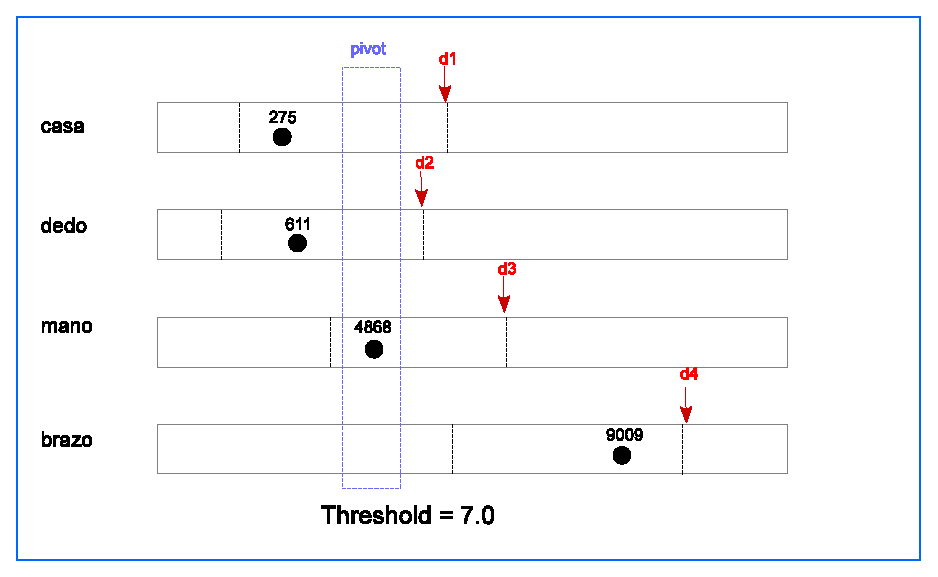
\includegraphics[scale=.75]{images/get_new_candidate.eps}
\caption{Ejemplo de cómo opera la functión getNewCandidate().}
\label{fig:getNewCandidate}
\end{figure}

\begin{algorithm}[!th]
\caption{\em $BMW(\theta, L, docID): Block Max Wand$}
\label{alg:bmw}
\begin{algorithmic}[1]
\REQUIRE Un \textit{threshold} $\theta$, listas invertidas $L$ de los términos en la consulta
\ENSURE $docID$, si existe un documento $docID$ tal que $score(docID)$ $\geq$ $\theta$. de lo contrario END-OF-FILE
\WHILE {true}
	\STATE $Sort(L);$
	\STATE $p = findPivot(L,\theta);$
	\STATE $d = L[p] \rightarrow currentDoc;$
	\IF {$d == $ END-OF-FILE}
  		\STATE $break;$
	\ENDIF
		
	\FOR {$ i = 0...p $}
		\STATE $NextShallow(d, L[i]);$
	\ENDFOR
	
	\IF {$isRealPivot(\theta, p);$}
		\IF {$L[0] \rightarrow currentDoc == d$}
			\STATE $scoreDoc(d, p);$
			\FOR {$ i = 0...p $}
				\STATE $Next(d + 1, L[i]);$
			\ENDFOR
		\ELSE
			\WHILE {$List[p - 1] \rightarrow currentDoc == p $}
				\STATE $p = p - 1;$			
			\ENDWHILE
			
			\FOR {$ i = 0...p $}
				\STATE $Next(d, L[i]);$
			\ENDFOR
			
		\ENDIF		
	\ELSE	
		\STATE $d' = getNewCandidate();$
		\FOR {$ i = 0...p $}
			\STATE $Next(d', L[i]);$
		\ENDFOR
	\ENDIF
	
\ENDWHILE

\end{algorithmic}
\end{algorithm}
\chapter{Métodos de predicción de rendimiento}
\label{cap:prediccion}
Lograr bajos tiempos de respuesta para transacciones de lectura es uno de los principales objetivos en el diseño de un motor de búsqueda, ya que de esta forma se le puede entregar una respuesta oportuna al usuario. Aquellas transacciones de lectura que requieren una gran cantidad de tiempo en ser resueltas degradan considerablemente la satisfacción del usuario, y es por esto que las máquinas de búsqueda están optimizadas para reducir el percentil más alto de los tiempos (también llamado \textit{tail latency}) \citep{Jeon:2014}. Paralelizar el procesamiento de cada consulta es una solución promitente para reducir el tiempo de ejecución de estas \citep{Jeon:2013, Tatikonda:2011}, lo cual es posible gracias a los modernos procesadores que existen hoy en día que poseen múltiples núcleos, en donde se puede resolver una consulta paralelizando múltiples hilos de ejecución.

Conocer de antemano la eficiencia de una transacción de lectura es una ventaja muy importante, puesto que aquellas consultas que toman una mayor cantidad de tiempo en ser resueltas se les asigna un mayor número de hilos de ejecución para resolverla, de esta manera se reduce el tiempo de procesamiento de las consultas y se cumple con la cota superior de tiempo establecida. Permite implementar técnicas efectivas de procesamiento y de planificación de transacciones de lectura, por ejemplo, en el contexto de procesamiento paralelo de consultas por lotes (\textit{batches}), se pueden crear grupos de consultas que posean similares tiempos de respuesta, así se tiende a disminuir tanto el desbalance de carga entre los procesadores como el tiempo en procesar el lote completo.

Con el objetivo de construir estrategias de procesamiento y planificación de consultas eficientes, en el presente trabajo se lleva a cabo la implementación de dos métodos de predicción de rendimiento para transacciones de lectura. La construcción de estos métodos de predicción se lleva a cabo con el objetivo de disminuir el tiempo en resolver conjuntos de consultas y asegurar una cota superior de tiempo para cada una de ellas. Adicionalmente, se busca estudiar cómo estos métodos afectan el rendimiento de un motor de búsqueda bajo el contexto de procesamiento de consultas por lotes utilizando el método Wand \citep{Broder:2003} y Block Max Wand \citep{Ding:2011}.

\section{Método de predicción multilineal}
\label{scheduling:glasgow}
Este método predice el tiempo de respuesta de una transacción de lectura y está basado en una regresión lineal múltiple con 42 variables independientes \citep{Macdonald:2012}. Como la respuesta a una consulta debe ser rápida, los estadísticos obtenidos desde las listas invertidas son previamente calculados en la fase de indexamiento, y en ningún caso es parte del proceso de resolución de la consulta. Los puntajes de los documentos son obtenidos mediante el método de \textit{ranking} BM25. 

Si bien es cierto que la regresión lineal posee 42 variables independientes, desde las listas invertidas se extraerán solo 14 estadísticos, ya que las 42 variables independientes se forman aplicando funciones de agregación sobre estos estadísticos. El estudio y el análisis estadístico de cada una de las variables involucradas en la regresión y su impacto en el tiempo está disponible en \citep{Macdonald:2012, Hauff:2010, He:2004}. A continuación se describe cada uno de los estadísticos $s(t)$ calculados en el proceso de indexamiento \citep{Croft:2009} de un sistema de recuperación de información.


\begin{list}{}{}
	\item \textbf{Media aritmética}. La media aritmética del puntaje de los documentos.

	\item \textbf{Media geométrica}. La media geométrica del puntaje de los documentos.

	\item \textbf{Media harmónica}. La media harmónica del puntaje de los documentos. 

	\item \textbf{Máximo puntaje}. Se obtiene el puntaje máximo perteneciente a algún documento dentro de la lista invertida. En otras palabras, se obtiene el \textit{upper bound} $UB_t$ de la lista. 

	\item \textbf{Varianza del puntaje}. Se extrae desde la lista invertida del término $t$, la varianza del puntaje de los documentos. 
	
	\item \textbf{Número de documentos}. Largo de la lista invertida. 

	\item \textbf{Número de maximos}. Número de veces en que aparece un nuevo puntaje máximo, es decir, el número de veces en que el \textit{upper bound} es actualizado. 

	\item \textbf{Número de documentos mayor a la media}. Número de documentos con puntaje superior al puntaje promedio. 
	
	\item \textbf{Número de documentos con puntaje máximo}. Número de documentos que poseen el puntaje máximo en la lista invertida del término $t$. 
	
	\item \textbf{Número de documentos dentro del 5\% más alto}. Número de documentos cuyos puntajes están dentro del 5\% superior. 
	
	\item \textbf{Número de documentos dentro del 5\% del umbral (\textit{threshold})}. Número de documentos cuyos puntaje están dentro del 5\% superior o 5\% inferior al \textit{threshold}. Recordar que el \textit{threshold} es el puntaje más bajo dentro del conjunto de \textit{top-K}.
	
	\item \textbf{Número de inserciones en el conjunto de los mejores $K$ documentos}. Para obtener este estadístico se asume que el término $t$ es una consulta con un solo término, se resuelve esta consulta con el método Wand y se calcula el número de inserciones de documentos que se hizo al \textit{heap}. Recordar que las inserciones al \textit{heap} ocurren cuando el puntaje completo del documento, supera al \textit{threshold}.
	
	\item \textbf{Frecuencia inversa de documento del término}. Se calcula el \textit{idf} del término $t$ \citep{Baeza-Yates:2011}.
	
	\item \textbf{Tiempo en ser procesado el término}. Tiempo que toma en ser procesado el término como si fuese una consulta de un solo término.

\end{list}

Los 14 estadísticos descritos anteriormente son la base para la implementación del predictor y estos son calculados por cada término del índice invertido. Adicionalmente se definen tres funciones de agregación que se usarán por cada consulta: máximo, varianza y suma. El proceso es el siguiente, para cada consulta que llega al sistema, se toman los 14 estadísticos de cada uno de los términos que la conforman, luego se aplican las funciones de agregación a los estadísticos de los términos. Por ejemplo, suponga que llegan dos consultas al sistema $q_1$ y $q_2$, ambas tendrán asociadas un vector de 14 estadísticos $E_{q_1}$ y $E_{q_2}$ respectivamente, las funciones de agregación para el estadístico de la media aritmética será calculado como sigue: $e_1 = max\{E_{q_1}(0), E_{q_2}(0)\}$, $e_2 = var\{E_{q_1}(0), E_{q_2}(0)\}$, $e_3 = sum\{E_{q_1}(0), E_{q_2}(0)\}$. De esta forma, con solo el primer estadístico (la media aritmética) se obtienen tres variables independientes ($e_1$, $e_2$, $e_3$). Si esto se extrapola a cada estadístico, se obtienen los 42 requeridos por el método. 
La Tabla \ref{tabla:estadisticosGlasgow} muestra un resumen de lo escrito anteriormente en donde se muestra cada uno de los estadísticos y los agregadores a utilizar. 

\begin{table}[!ht]
\centering
\caption{Resumen de los estadísticos para la predicción multilineal}
\begin{tabular}{|l|}
\hline
\multicolumn{1}{|c|}{Estadísticos de términos $s(t)$} \\ \hline
1. Media aritmética \\ 
2. Media geométrica \\ 
3. Media harmónica \\ 
4. Puntaje máximo \\ 
5. Varianza del puntaje \\ 
6. Número de documentos \\ 
7. Número de máximos \\ 
8. Número docs $>$ media \\ 
9. Número docs = máximo puntaje \\ 
10. Número docs dentro del 5\% más alto \\
11. Número docs dentro del 5\% del \textit{threshold} \\ 
12. Número de inserciones al conjunto \textit{top-K} \\ 
13. IDF \\ 
14. Tiempo en resolver $t$ como consulta \\ \hline
\multicolumn{1}{|c|}{Agregadores A()} \\ \hline
a. Máximo \\ 
b. Varianza  \\ 
c. Suma \\ \hline
\end{tabular}
\label{tabla:estadisticosGlasgow}
\end{table}

\section{Método de predicción neuronal}
\label{scheduling:neuronal}
Se implementa un método de predicción basado en una red neuronal \textit{backpropagation} \citep{Rumelhart:1988}. La característica de este tipo de redes es que utilizando al menos una capa oculta, se puede aproximar cualquier tipo de función o relación continua entre un grupo de variables de entrada y salida. Este tipo de redes neuronales utilizan un método de entrenamiento en el cual se propaga el error hacia atrás para ajustar los pesos de las diferentes neuronas del modelo, de esta forma la red neuronal va generando una asociación entre la entrada y salida \citep{Fausett:1994}.

Se implementa el modelo neuronal usando las mismas 42 variables independientes del método anterior, debido a que ya se ha demostrado que existe una relación lineal entre estas variables y la variable tiempo \citep{Macdonald:2012, Hauff:2010, He:2004}. El modelo consiste de dos neuronas en una capa oculta, la idea es que el tiempo que toma la predicción no genere un impacto negativo en el tiempo de procesamiento de la consulta, es por esto que se decide utilizar solo dos neuronas, sin embargo, en el Capítulo \ref{cap:evaluacionexperimental} también se hace un análisis del modelo con 10 y 20 neuronas en la capa oculta. El objetivo es minimizar el error de la estimación de tiempo y que la predicción no genere un impacto negativo en términos de tiempo.
\chapter{Estrategias de planificación de queries}
\label{cap:planificacion}

Nosotros optamos por un enfoque de Wand Heap Compartido para ser usado en los experimentos.

Se habla de enfoque de bloques también.

Recordar el contexto de planificación de queries y ejecución de queries.

\section{Estrategias por bloques}
\label{scheduling:bloques}

Hablar sobre las estrategias por bloques

Se utilizará predictor de tiempo para setear threads

Se muestra scheduler.odg para el esquema de forma general

La estrategia teorica FR presentada en (citar) que estudia X, dio pie a la propuesta de... 
La estrategia de planificación FR es un algoritmo teórico de planificación de trabajos paralelos (parallel job) que llegan al sistema uno a uno \citep{Ye:2007}.


\subsection{Estrategia FR}
\label{scheduling:fr}
La estrategia de planificación FR asume que cada query que llega al motor de búsqueda posee el tiempo en que se domorará en ser procesada. 

Sehace una clsificación de las queries entre Big y Small con el objetivo de crear estructuras de datos denominadas Rooms y Walls, en donde Walls y Tooms estarán formadas por queries Bigs y Smalls respectivamente. Ambas estructuras tienen un número máximo de máquinas disponibles para procesar las queries. Una consulta es Big si el número de máquinas requeridas para procesarlas es m (siendo m el número de máquinas disponibles),, de lo contrario, la query es small. 
% Debe estar bloqueada porque eventualmente el ejecutador de queries estará sacando

% ----  Descripción del algoritmo ----
Como se puede ver en el Algoritmo \ref{alg:fr}, cuando una nueva query llega al sistema se analiza si esta es de tipo Big o Small; esto se hace en el método isBig(), que retorna verdadero si es que el número de máquinas requeridas para procesarla es igual al máximo de máquinas disponibles, de lo contrario retorna falso. Si la consulta es big, entonces se crea un nuevo Wall, se agrega la query al bloque y el bloque es planificado en la lista de planificación SchedulingList. Si se está en presencia de una transacción de lectura Small, entonces se busca algún bloque disponible para planificar la query, esto se hace desde el primer bloque abierto para recibir transacciones de lectura hasta el final de la schedulingList. Finalmente, si es eventualmente no se encuentra algún bloque disponible para planificar la query, entonces se crea un nuevo bloque Room, se asigna la consulta al bloque y se asigna el bloque a la lista de scheduling. Cabe destacar que se dice que un bloque está abierto cuando (isOpen) cuando aún le quedan máquinas disponibles o cuando el proceso de ejecución ya ha tomado las queries de este bloque para resolverlas.
%----- Fin descripción algoritmo ----

\begin{algorithm}[!th]
\caption{\em $assignQuery(L, Q)$: Planificación de consulta}
\label{alg:fr}
\begin{algorithmic}[1]
\REQUIRE Una SchedulingList $L$ en donde se hará la planificación, QueryObject $Q$ a planificar
\ENSURE SchedulingList $L$ con la nueva query planificada

\IF {$isBig(query)$}
	\STATE $block = new Wall();$
	\STATE $block \rightarrow addQuery(query);$
	\STATE $L \rightarrow addBlock(block);$
\ELSE
	\STATE $asignada = false;$
	\FOR {$ i = L \rightarrow firstOpenBlockLocked()...L \rightarrow sizeLocked()$}
		\STATE $room\_block = L \rightarrow getBlockLocked(i);$
		
		\IF {$(room\_block \rightarrow isOpen()) AND 
				(room\_block \rightarrow freeThreads() >= query \rightarrow getThreads())$
			}
			\STATE $room\_block \rightarrow addQuery(query)$
			\STATE $asignada = true$
			\STATE $break;$
		\ENDIF
	\ENDFOR
	
	\IF {$!(asignada)$}
		\STATE $block = new Room();$
		\STATE $block \rightarrow addQuery(query);$
		\STATE $L \rightarrow addBlockLocked(block);$		
	\ENDIF
\ENDIF

\end{algorithmic}
\end{algorithm}


// Esquema de ejecución

// Algoritmo

// Ejemplo de cómo van quedando los bloques



\section{Estrategia \textit{1TQ}}
\label{scheduling:baseline}
Un simple camino para construir un sistema que responda a múltiples consultas simultáneamente usando múltiple hilos de ejecución, es usando estos hilos de manera independiente. Para hacer esto se debe mantener un conjunto de \textit{threads} consumidores que trabajarán en paralelo y se encargarán de resolver las \textit{queries} secuencialmente (una a una) desde una misma cola, esto es lo que en este trabajo se denomina estrategia de Un Thread Por Query (1TQ). En la Figura \ref{fig:1TQ} se puede apreciar el esquema de ejecución en donde cada uno de los procesos genera una petición de alguna consulta en la cola, si quedan \textit{queries} por procesar entonces se le asigna al proceso una consulta que tendrá que resolver de manera secuencial. Se debe tener en cuenta que cada vez que un proceso genera una solicitud de \textit{query}, se bloquea la estructura de datos que contiene las consultas a procesar y luego se procesa la solicitud, de esta forma se asegura un acceso seguro por parte de los distintos \textit{threads}. 

\begin{figure}[H]
\centering
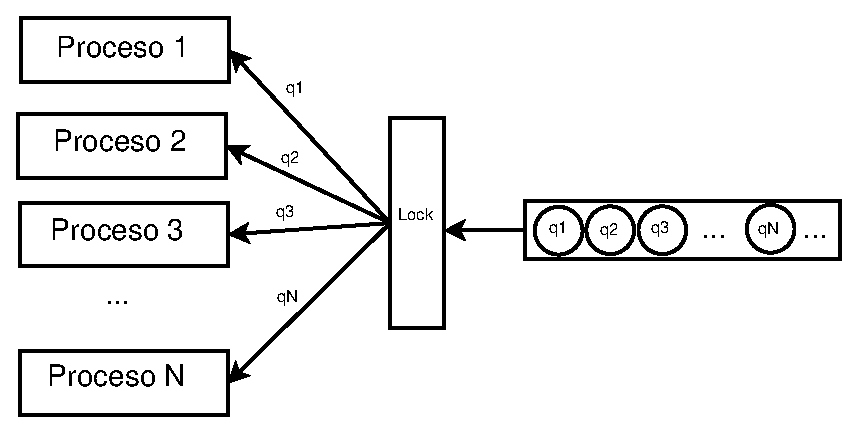
\includegraphics[scale=.75]{images/1TQ.eps}
\caption{Ejemplo de procesamiento estrategia 1TQ}
\label{fig:1TQ}
\end{figure}

Este esquema tiene la ventaja que es simple y fácil de implementar y controlar. Sin embargo, existen sistemas de recuperación de la información como los motores de búsqueda verticales que cuando están ejecutando \textit{batches} de \textit{queries} deben parar su ejecución porque transacciones de escritura han llegado al sistema, y este deben actualizar la información del índice invertido. Solo después de la fase de actualización el sistema es capaz de ejecutar el siguiente \textit{batch} de transacciones de lectura. Al final de cada conjunto de consultas, es posible que algunos hilos de ejecución del sistema finalicen su trabajo y que no tengan más \textit{queries} para procesar, por lo que ellos tienen que esperar que los \textit{threads} restantes finalicen su trabajo antes que el sistema entre en la fase de actualización de su índice invertido o bien, se pase a la ejecución del siguiente \textit{batch} de consultas.
Sin embargo, aunque cada hilo de ejecución está secuencialmente ejecutando una transacción de lectura diferente, algunas de estas operaciones puede tomar un tiempo cosiderable, de esta forma se produce una importante pérdida de eficiencia, aunque la intuición nos dice que esto se puede mitigar con \textit{queries} que requieran poca cantidad de tiempo para ser procesada (trabajos pequeños o \textit{small jobs}). 
En la Figura \ref{fig:small_jobs} queda reflejado lo dicho en el párrafo anterior. Si los trabajos que cada \textit{thread} está ejecutando son pequeños, entonces probablemente la pérdida de trabajo al final de cada \textit{batch} de consultas será menor al trabajo que se pierde cuando los trabajos son grandes (ver Figura \ref{fig:large_jobs}).  


\begin{figure}[H]
\centering
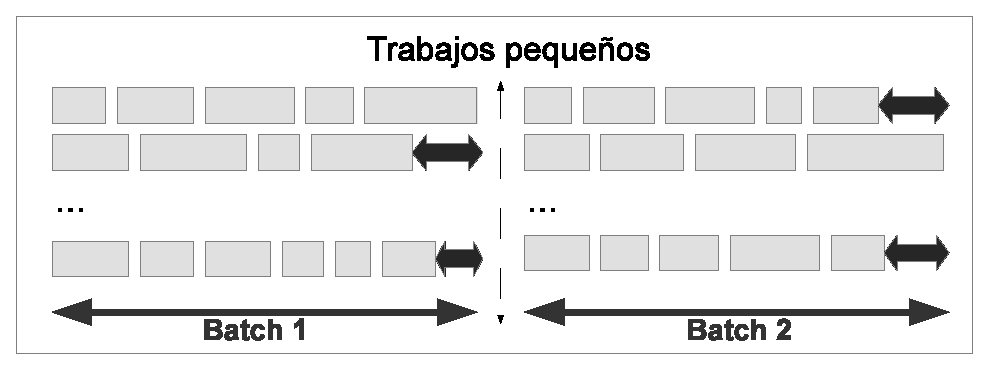
\includegraphics[scale=.75]{images/small_jobs.eps}
\caption{Ejecución en paralelo de \textit{small jobs}}
\label{fig:small_jobs}
\end{figure}

\begin{figure}[H]
\centering
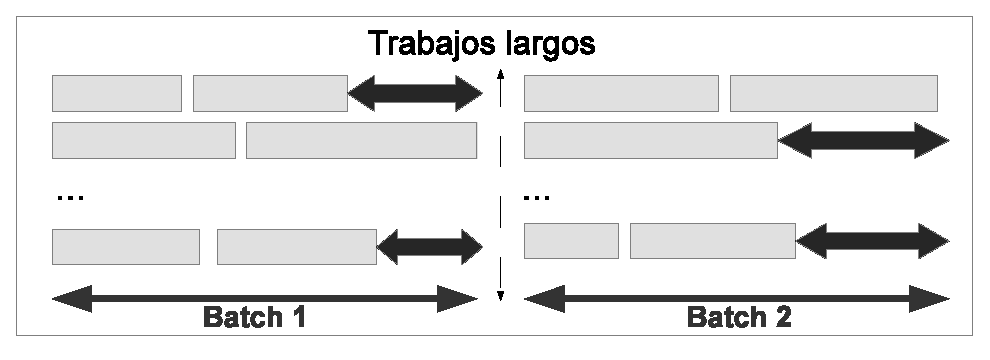
\includegraphics[scale=.75]{images/large_jobs.eps}
\caption{Ejecución en paralelo de \textit{large jobs}}
\label{fig:large_jobs}
\end{figure}



\section{Estrategia unidades de trabajo}
\label{scheduling:unidadestrabajo}
Con respecto a los esquemas explicados hasta ahora, el esquema 1TQ tiene la ventaja que no solo requiere menos control, sino que también permite a los hilos de ejecución trabajar sin pausa mientras un \textit{batch} de consultas está siendo procesado. En esta sección se propone un esquema híbrido basado en unidades de procesamiento (\textit{Processing Units}) que aproveche las ventajas de ambos enfoques. (se requiere ver el tema de bloques).
En este nuevo esquema de planificación, las consultas pasan a través de una fase en la cual cada \textit{query} es evaluada y se determina un apropiado número de unidades de procesamiento (\textit{processing units}) para poder resolver dicha consulta. Este proceso es llevado a cabo de manera similar al proceso en donde se determina la cantidad de \textit{threads} apropiados para resolver una determina transacción de lectura. Este número de unidades de procesamiento es creado y asociado a cada consulta, finalmente se guarda en una cola de unidades de trabajo. Un conjunto de \textit{threads} consumidores extraen las unidades desde la cola y las procesa independientemente. Cuando un \textit{thread} finalice el procesamiento de la unidad de trabajo actual automáticamente leerá la siguiente unidad de trabajo desde la cola. 
Generalmente lo que se hace habitualmente es estimar el número de \textit{threads} con el que se resolverá la consulta, como se muestra en la Figura \ref{fig:unit_process} en este nuevo enfoque se intenta estimar el número de unidades de trabajo con el que se resolverá cada consulta. Además, se debe controlar el acceso concurrente de los hilos de ejecución a la cola de unidades de trabajo, de tal manera que solo un thread tenga acceso exclusivo a la estructura de datos. 

\begin{figure}[!th]
\centering
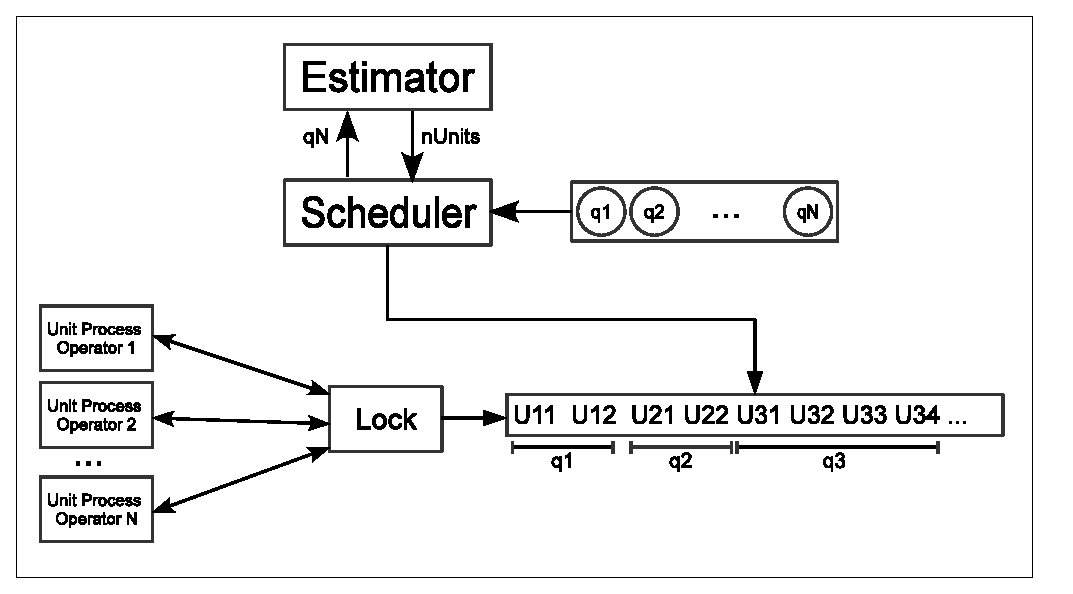
\includegraphics[scale=.75]{images/unit_process.eps}
\caption{Procesamiento de consultas utilizando unidades de trabajo}
\label{fig:unit_process}
\end{figure}

El procesamiento de cada hilo de ejecución es una versión de Wand con heap compartido (SH), adaptado de manera tal que cada unidad de trabajo es resuelta independientemente de si existen otras unidades siendo procesada al mismo tiempo o no. La única excepción es que la unidad que inicializa la consulta es siempre ejecutada antes del resto de las otras unidades de la misma consulta y la entrega de resultados se hace una vez que todas las unidades de trabajo de la \textit{query} han finalizado. Este enfoque híbrido permite reducir el tiempo perdido al final de cada \textit{batch} sin generar una importante pérdida de trabajo mientras las \textit{queries} del \textit{batch} están siendo procesadas.

\chapter{Evaluación experimental}
\label{cap:evaluacionexperimental}
En el presente capítulo se presenta los resultados obtenidos de las diferentes implementaciones para los métodos propuestos en la secciones anteriores. Se comienza por la implementación de los métodos de procesamiento de transacciones de lectura, posteriormente se muestra los resultados obtenidos para los diferentes métodos de predicción de tiempos de respuestas para consultas y el comportamiento que tienen para diferente conjunto de datos. Finalmente se presenta el comportamiento de las estrategias de planificación presentadas para diferentes tipos de escenarios.

\section{Hardware y conjunto de datos}
\label{evaluacionexperimental:hardwareydatos}
Los experimentos fueron ejecutados en un Intel Xeon E5620 2.4 \textit{Ghz.} con 8 núcleos físicos, tecnología \textit{hyper-threading} y 90 gigabytes de memoria de acceso aleatorio (\textit{RAM}). Se utilizaron dos conjuntos de datos para llevar a cabo los experimentos, estos son frecuentemente usados por la comunidad del área de Information Retrieval. El primero de ellos es \textit{GOV2}, este conjunto es una colección de aproximadamente 25 millones de páginas \textit{Web} obtenida desde los dominios \textit{.gov} y que pesa 426 \textit{GB}. La otra colección de datos utilizada es la \textit{ClueWeb09}, la cual fue creada para apoyar la investigación en recuperación de la información y las tecnologías relacioanadas con el lenguaje humano, consiste en alrededor de un billón de páginas en diez lenguajes diferentes y 50 millones en inglés. \textit{ClueWeb09} pesa alrededor de 5 \textit{TB} en forma comprimidad y 25 \textit{TB} descomprimida. 
% Las consultas (queries)

\section{Wand multithreaded}
\label{evaluacionexperimental:wm}
En esta sección se muestra la implementación de dos enfoques para el procesamiento de consultas a través del algoritmo Wand \citep{Broder:2003}. El primer enfoque es el esquema de \textit{heap} locales (LH), en el que cada hebra obtiene sus mejores documentos para una consulta dada y luego una hebra maestra se encarga de mezclar todos los resultados de cada uno de los hilos de ejecución para construir el conjunto \textit{top-K} final; el segundo enfoque es el enfoque de \textit{heap} compartido (SH), en el que se tiene un \textit{heap} visible a todos los hilos de ejecución y en donde ellos compiten por el acceso a esta estructura de datos. El detalle del diseño de los enfoques LH y SH están disponibles en \ref{scheduling:wlh} y \ref{scheduling:whc}. 

\subsection{Esquema LH}
\label{evaluacionexperimental:esquemalh}
En el esquema LH todos los hilos de ejecución tienen sus propias estructuras de datos y variables que soportan la resolución de una transacción de lectura. La clase \textit{TopKMultithreadWandOperatorLocal} es la encargada de administrar la lógica de ejecución, además prepara las variables e inicia los hilos de ejecución. El Código \ref{code:topkmultithreadwandoperatorlocal} muestra la implementación, en el que existe un método llamado \textit{execute}, este método es el encargado de llevar a cabo la resolución de la consulta, recibe como entrada la consulta a ser resuelta y un vector de resultados, en el que se almacenará los resultados obtenidos. Adicionalmente, este método es el encargado de lanzar las hebras con que se resolverá cada consulta y a cada uno de ellas le asiga un objeto de tipo \textit{TopKWandOperator} ($arr\_ops[pid\_thread]$) para obtener los resultados. Todo este proceso es llevado a cabo usando $K$ como tamaño del conjunto que se quiere obtener. Además se definen variables como \textit{$mapas\_ubs$}, el cual asocia a cada término los \textit{upper bounds} con los que el método Wand trabajará y \textit{$query\_partes$}, variable que define en cuántas partes la consulta debe ser dividia y está supeditada al número de hebras con que esta será resuelta.

\lstinputlisting[label=code:topkmultithreadwandoperatorlocal, caption=Implementación de la clase TopKMultithreadWandOperatorLocal.h, language=C++]{code/TopKMultithreadWandOperatorLocal.h}

En la Figura \ref{fig:esquema_ejecucion_wandsh} se ejemplifica la resolución de una consulta con cuatro hilos de ejecución. Una vez que el sistema asigna el número de hebras que se utilizará para la resolución de la consulta, esta es tomada por el objeto \textit{TopKMultithreadWandOperatorLocal} y hace un llamado al método \textit{execute}, en el que se hace una preparación de variables y se lanzan los hilos de ejecución; cada uno de ellos tiene asignado dos objetos: (1) \textit{TopKWandOperator}, el cual se encarga de que cada hilo de ejecución solo resuelva la parte de la consulta que se le asignó, y (2) \textit{Wand}, el cual se encarga de obtener los mejores $K$ documentos guardándolos en un \textit{heap}.

\begin{figure}[th!]
\centering
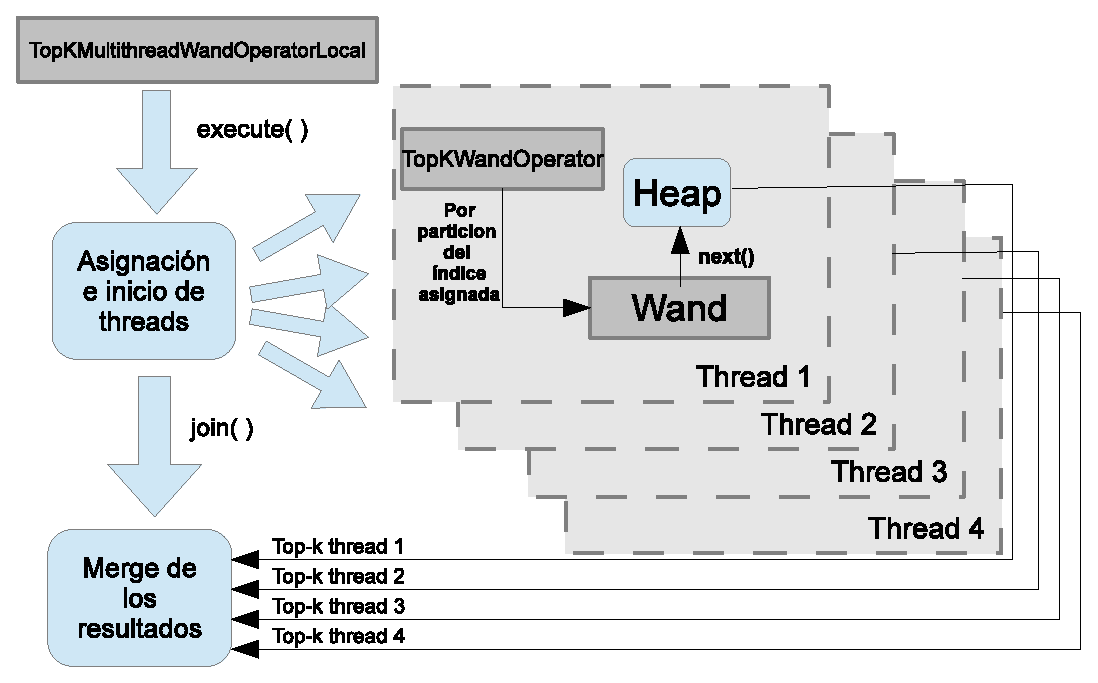
\includegraphics[scale=.75]{images/ejecucion_topkmultithreadwandopLOCAL.eps}
\caption{Esquema de ejecución enfoque LH}
\label{fig:esquema_ejecucion_wandlh}
\end{figure}

\subsection{Esquema SH}
\label{evaluacionexperimental:esquemash}
En el esquema SH los hilos de ejecución trabajan con variables compartidas, incluído el \textit{heap} en donde se almacenan los resultados. La ejecución de este enfoque es llevada a cabo por la clase \textit{TopKMultithreadWandOperatorLocks}, la cual podemos ver en el Código \ref{code:topkmultithreadwandoperatorlocks}; en esta implementación se puede observar la declaración de una clase anidada la que contiene las variables que serán compartidas por los hilos de ejecución. Dentro de las variables más importantes está el \textit{heap}, el umbral utilizado para decidir si un documento debe estar dentro del \textit{heap} y la variable de tipo \textit{mutex} que permite el acceso exclusivo a las variables compartidas. 

\lstinputlisting[label=code:topkmultithreadwandoperatorlocks, caption=Implementación de la clase TopKMultithreadWandOperatorLocks.h, language=C++]{code/TopKMultithreadWandOperatorLocks.h}

La Figura \ref{fig:esquema_ejecucion_wandsh} muestra un ejemplo de resolución de consulta utilizando cuatro hilos de ejecución y el enfoque SH. Al igual que en el esquema anterior, la clase principal inicializa variables e inicia los hilos de ejecución; el objeto \textit{TopKWandOperator} asignará a cada hebra la parte del índice invertido con la que cada hebra resolverá la consulta. Cada vez que un hilo de ejecución utilizando el objeto Wand encuentre un documento candidato para estar en el conjunto \textit{top-K} final, debe pedir acceso exclusivo a las estructuras de datos involucradas (\textit{heap} y umbral), de esta forma se evita resultados erróneos en el conjunto final producto del paralelismo entre los hilos de ejecución.  

\begin{figure}[th!]
\centering
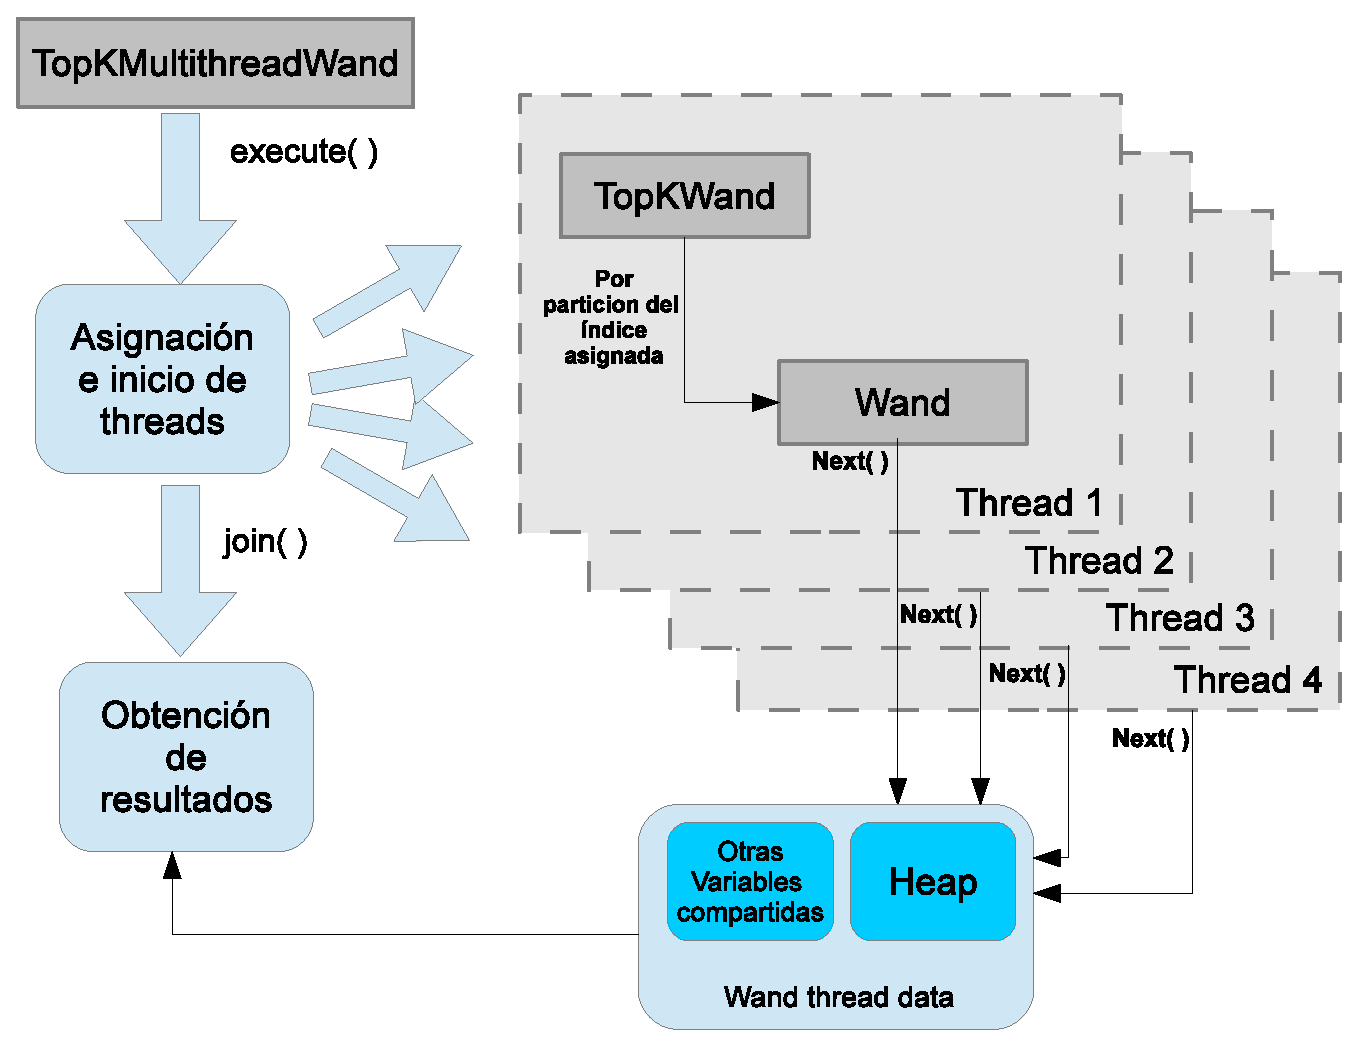
\includegraphics[scale=.75]{images/ejecucion_topkmultithreadwandopCOMPARTIDO.eps}
\caption{Esquema de ejecución enfoque SH}
\label{fig:esquema_ejecucion_wandsh}
\end{figure}


\subsection{Resultados obtenidos}
\label{evaluacionexperimental:resultadosObtenidos}
En la Figura \ref{fig:tiempos_wand} se puede observar el tiempo promedio del enfoque LH y el enfoque SH en resolver un conjunto de 10,000 consultas de la colección \textit{GOV2}. A medida que crece el número de hilos de ejecución, el enfoque de \textit{heaps} compartidos toma ventaja por sobre el enfoque de \textit{heaps} locales, sin embargo, cuando se utiliza un hilo de ejecución se puede observar que LH ($117.486 ms$) requiere un tiempo menor que SH ($130.591 ms$), esto se debe porque en LH no se usa variables compartidas que retrase a los hilos de ejecución esperando a que otros las libere. LH requiere menos tiempo en resolver el \textit{log} de consultas para 2,4,8 y 16 hebras. 
El esquema LH puede estar muy supeditado a la distribución de documentos en las listas del índice invertido, ya que si un hilo de ejecución procesa su corrrespondiente parte del índice invertido en donde los mejores puntajes se encuentran al final, entonces el \textit{heap} tendrá un umbral bajo al comienzo del proceso, eso implica un proceso de descarte de documentos menos eficiente y el tiempo de ejecución requerido será mayor, retrasando el proceso que mezcla los resultados para obtener el conjunto \textit{top-K} final. 
Como el esquema SH ocupa un solo \textit{heap} para obtener los mejores $K$ documentos, el \textit{heap} tiende a llenarse rápidamente con los mejores documentos globales, esto implica que el puntaje mínimo del \textit{heap} (umbral) tiende a crecer rápidamente, permitiendo un mejor descarte de documentos y menor tiempo de ejecución para las hebras. 

\begin{figure}[!ht]
\centering
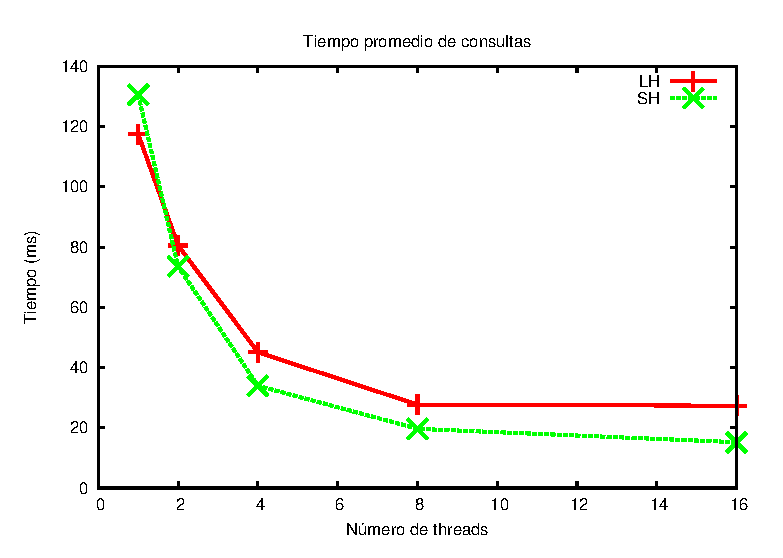
\includegraphics[scale=.75]{images/tiempos_wand.eps}
\caption{Tiempos promedios de las consultas}
\label{fig:tiempos_wand}
\end{figure}

Adicionalmente en la Figura \ref{fig:eficiencias_wand} se puede ver en forma general que con la estrategia de enfoques compartidos se obtiene mejores eficiencias que con la estrategia LH. Con SH la mejor eficiencia que se obtiene es con 4 hilos de ejecución ($0.962 ms$), mientras que con 2 y con 8 hebras se obtiene una eficiencia de $0.887$ y $0.831 milisegundos$; en general se obtiene buenas eficiencias para 1,2,4 y 8 hebras, sin embargo, con 16 hilos de ejecución la eficiencia baja considerablemente ($0.5403$) con respecto a las anteriores, esto se debe principalmente a la tecnología \textit{thyperthreading} de la máquina utilizada. También es interesante ver que el uso exclusivo del \textit{heap} compartido por parte de los \textit{threads} no tiene un fuerte impacto en el rendimiento. La eficiencia baja de LH se debe porque para obtener el conjunto \textit{top-K} final de una consulta debe haber una sincronización de todos los hilos de ejecución involucrados en que cada uno de ellos envíe sus \textit{top-K} locales a la hebra maestra, y además porque existe un costo adicional de calcular el conjunto \textit{top-K} final entre los $P \times K$ documentos seleccionados (siendo $P$ el número de procesadores). 
                     
%Para los siguientes experimentos del presente trabajo se ocupará el enfoque SH para resolver las transacciones de lectura.

\begin{figure}[!ht]
\centering
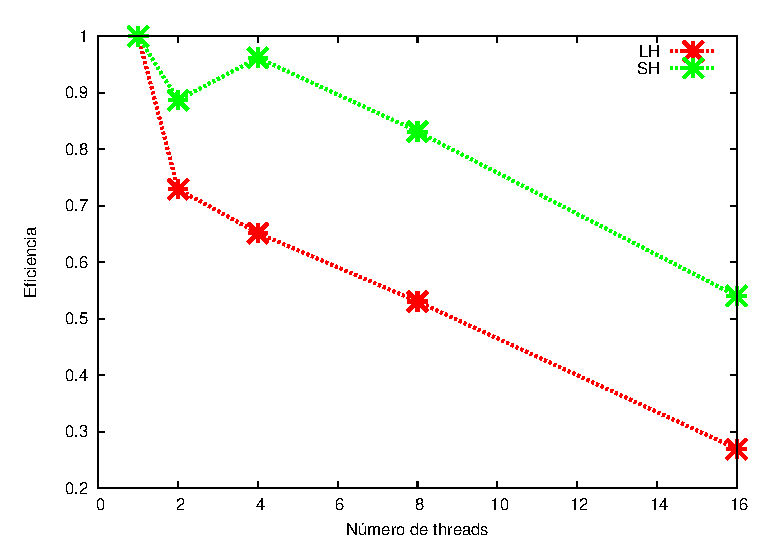
\includegraphics[scale=.75]{images/eficiencias_wand.eps}
\caption{Eficiencias para Wand con heaps compartido y locales}
\label{fig:eficiencias_wand}
\end{figure}

\section{Predicción de tiempos}
\label{evaluacionexperimental:predicciontiempos}


\section{Estrategias de scheduling}
\label{evaluacionexperimental:estrategiasscheduling}
\chapter{Conclusiones}
\label{cap:conclu}

Utilizando Wand y Gov2 Heap compartido > Heap global.

¿Comportamiento según Wand y Conjunto De Datos? 

El beneficio de la predicción de tiempo en el esquema de un solo procesador parece no ser beneficioso. 
El impacto que toma predecir el tiempo...

Las estrategias diseñadas fueron pensadas en el contexto en que al final de cada lote de consultas se produce una sincronización.

Se analizó algunas de las estrategias de planificaicón que hay en el estado del arte, se llevó al contexto practicó desarrollando tb un estimador de threads, pero al final del día se dio cuenta que el costo de predecir y el beneficio que entrega la planificación no son muy buenos.

Se traen estrategias del estado del arte, se adaptan, se comparan y se concluye algo.

ok, entonces es mejor usar este enfoque de unidades

se analizan los resultados de cada uno de los algoritmos

Trabajo futuro, probar con diferentes K, probar reducir el modelo lineal, probar otras estrategias de planificación.
% ----------------------------------------------------------
\bibliographystyle{apa-good}
\bibliography{referencias}
% ----------------------------------------------------------
% NO TIENE APENDICES
\appendix
\addappheadtotoc 
% ----------------------------------------------------------
\chapter{Resultados del proceso de entrenamiento}
\label{ape:apeA}

\begin{table}[htbp]
\caption{Resultados método ML utilizando el conjunto de datos Gov2 y método de procesamiento Block Max Wand.}
\begin{center}
\begin{tabular}{|c|c|c|c|c|c|}
\hline
\multicolumn{ 6}{|c|}{Estimador ML – GOV2 – BMW} \\ \hline
 & 1 thread & 2 threads & 4 threads & 8 threads & 16 threads \\ \hline
r & \multicolumn{1}{r|}{0,8782952873} & \multicolumn{1}{r|}{0,8809618279} & \multicolumn{1}{r|}{0,8479348273} & \multicolumn{1}{r|}{0,7771884041} & \multicolumn{1}{r|}{0,7377811742} \\ \hline
RMSE & 72,364708101 & 40,8927943754 & 20,1217578763 & 13,7608115407 & 12,4521027766 \\ \hline
\end{tabular}
\end{center}
\label{ml_gov2_bmw}
\end{table}

\begin{table}[htbp]
\caption{Resultados método ML utilizando el conjunto de datos ClueWeb y método de procesamiento Wand.}
\begin{center}
\begin{tabular}{|c|c|c|c|c|c|}
\hline
\multicolumn{ 6}{|c|}{Estimador ML – ClueWeb – WAND} \\ \hline
 & 1 thread & 2 threads & 4 threads & 8 threads & 16 threads \\ \hline
r & 0,8613156155 & 0,8726350536 & 0,8646059611 & 0,8598639269 & 0,8497258186 \\ \hline
RMSE & 91,9765237227 & 48,1189862101 & 21,9652740764 & 12,1717738001 & 9,3846426006 \\ \hline
\end{tabular}
\end{center}
\label{ml_clueweb_wand}
\end{table}

\begin{table}[htbp]
\caption{Resultados método ML utilizando el conjunto de datos ClueWeb y método de procesamiento Block Max Wand.}
\begin{center}
\begin{tabular}{|c|c|c|c|c|c|}
\hline
\multicolumn{ 6}{|c|}{Estimador ML - ClueWeb – BMW} \\ \hline
 & 1 thread & 2 threads & 4 threads & 8 threads & 16 threads \\ \hline
r & 0,8828211665 & 0,8891976969 & 0,808606576 & 0,823249926 & 0,7451258225 \\ \hline
RMSE & 64,7039723565 & 35,281001295 & 25,7540777939 & 15,8306946733 & 17,9398672123 \\ \hline
\end{tabular}
\end{center}
\label{ml_clueweb_bmw}
\end{table}

% ----------------- Redes neuronales -------------------

\begin{table}[htbp]
\caption{Resultados método RN utilizando el conjunto de datos Gov2 y método de procesamiento Block Max Wand.}
\begin{center}
\begin{tabular}{|c|c|c|c|c|c|}
\hline
\multicolumn{ 6}{|c|}{Estimador RN – GOV2 – BMW} \\ \hline
 & 1 thread & 2 threads & 4 threads & 8 threads & 16 threads \\ \hline
r & 0,932476451 & 0,9360700621 & 0,8966995703 & 0,827613008 & 0,7880014511 \\ \hline
RMSE & 54,7912225707 & 82,2905244753 & 60,3315527261 & 21,882569362 & 5,7758056986 \\ \hline
\end{tabular}
\end{center}
\label{rn_gov2_bmw}
\end{table}

\begin{table}[htbp]
\caption{Resultados método RN utilizando el conjunto de datos Clueweb y método de procesamiento Wand.}
\begin{center}
\begin{tabular}{|c|c|c|c|c|c|}
\hline
\multicolumn{ 6}{|c|}{Estimador RN – ClueWeb – Wand} \\ \hline
 & 1 thread & 2 threads & 4 threads & 8 threads & 16 threads \\ \hline
r & 0,9214415134 & 0,928326314 & 0,9547375955 & 0,9520042927 & 0,9498575917 \\ \hline
RMSE & 70,5610058313 & 98,6489306355 & 65,1112021339 & 24,172402818 & 8,4319553251 \\ \hline
\end{tabular}
\end{center}
\label{rn_clueweb_wand}
\end{table}

\begin{table}[htbp]
\caption{Resultados método RN utilizando el conjunto de datos Clueweb y método de procesamiento Block Max Wand.}
\begin{center}
\begin{tabular}{|c|c|c|c|c|c|}
\hline
\multicolumn{ 6}{|c|}{Estimador RN – ClueWeb – BMW} \\ \hline
 & 1 thread & 2 threads & 4 threads & 8 threads & 16 threads \\ \hline
r & 0,9583572968 & 0,9581178412 & 0,8717897021 & 0,9019796766 & 0,8192397311 \\ \hline
RMSE & 39,546150466 & 75,4843974473 & 48,4467865615 & 24,9504558614 & 17,0429025714 \\ \hline
\end{tabular}
\end{center}
\label{rn_clueweb_bmw}
\end{table}
\chapter{Resultado del proceso de evaluación de los modelos de aprendizaje}
\label{ape:apeB}

\begin{table}[htbp]
\caption{Errores obtenidos método ML utilizando Gov2 y Wand}
\begin{center}
\begin{tabular}{|c|c|c|c|c|c|}
\hline
 & \multicolumn{ 5}{c|}{Estimador ML - Gov2 Test – Wand} \\ \hline
 & 1t & 2t & 4t & 8t & 16t \\ \hlin
RMSE ML & 93,4213321631 & 55,2226746394 & 35,8065152454 & 31,5809909101 & 30,9943417318 \\ \hline
ERP ML (\%) & 46,7679492043 & 48,3620334358 & 49,158464109 & 54,3328274289 & 54,4780442408 \\ \hline
\end{tabular}
\end{center}
\label{ml_gov2test_wand}
\end{table}

\begin{table}[htbp]
\caption{Errores obtenidos método ML utilizando Gov2 y Block Max Wand.}
\begin{center}
\begin{tabular}{|l|c|r|r|r|r|}
\hline
 & \multicolumn{ 5}{c|}{Estimador ML - Gov2 Test – BMW} \\ \hline
 & 1t & \multicolumn{1}{c|}{2t} & \multicolumn{1}{c|}{4t} & \multicolumn{1}{c|}{8t} & \multicolumn{1}{c|}{16t} \\ \hline
RMSE ML & \multicolumn{1}{r|}{88,5781924513} & 50,2281785684 & 65,3589630276 & 85,0273335875 & 104,9557422762 \\ \hline
Error ML (\%) & \multicolumn{1}{r|}{40,9396043829} & 43,5946339982 & 57,8712066627 & 73,6999382771 & 80,2156076147 \\ \hline
\end{tabular}
\end{center}
\label{table:ml_gov2test_bmw}
\end{table}

\begin{table}[htbp]
\caption{Errores obtenidos método ML utilizando Clueweb y Block Max Wand.}
\begin{center}
\begin{tabular}{|l|c|r|r|r|r|}
\hline
 & \multicolumn{ 5}{c|}{Estimador ML – Clueweb Test – Wand} \\ \hline
 & 1t & \multicolumn{1}{c|}{2t} & \multicolumn{1}{c|}{4t} & \multicolumn{1}{c|}{8t} & \multicolumn{1}{c|}{16t} \\ \hline
RMSE ML & \multicolumn{1}{r|}{105,0379461837} & 55,108354518 & 32,3000081798 & 24,7425815335 & 29,7917310828 \\ \hline
Error ML (\%) & \multicolumn{1}{r|}{38,2730089817} & 37,9789108856 & 39,2179670254 & 40,2465224632 & 47,8721024955 \\ \hline
\end{tabular}
\end{center}
\label{table:ml_cluewebtest_wand}
\end{table}

\begin{table}[htbp]
\caption{Errores obtenidos método ML utilizando Clueweb y Block Max Block Max Wand.}
\begin{center}
\begin{tabular}{|l|c|r|r|r|r|}
\hline
 & \multicolumn{ 5}{c|}{Esimador ML – Clueweb Test – BMW} \\ \hline
 & 1t & \multicolumn{1}{c|}{2t} & \multicolumn{1}{c|}{4t} & \multicolumn{1}{c|}{8t} & \multicolumn{1}{c|}{16t} \\ \hline
RMSE ML & \multicolumn{1}{r|}{63,2614531088} & 35,318259738 & 19,7612998424 & 18,0902452623 & 21,9105063561 \\ \hline
Error ML (\%) & \multicolumn{1}{r|}{31,3197074579} & 32,8018021931 & 34,9491116301 & 33,1906288908 & 36,8597795426 \\ \hline
\end{tabular}
\end{center}
\label{table:ml_cluewebtest_bmw}
\end{table}

%---------- redes neuronales ahora
\begin{table}[htbp]
\caption{Errores obtenidos método RN utilizando Gov2 Test y Wand.}
\begin{center}
\begin{tabular}{|c|c|c|c|c|c|}
\hline
 & \multicolumn{ 5}{c|}{Estimador RN - Gov2 - Wand} \\ \hline
 & 1t & 2t & 4t & 8t & 16t \\ \hline
RMSE RN & 83,3427688489 & 127,7971510158 & 78,5508679211 & 44,0078238263 & 32,5958111096 \\ \hline
ERP RN (\%) & 39,6467173103 & 109,5123072913 & 141,1360887399 & 123,600300482 & 62,1680304214 \\ \hline
\end{tabular}
\end{center}
\label{rn_gov2test_wand}
\end{table}

\begin{table}[htbp]
\caption{Errores obtenidos método RN utilizando Gov2 Test y Block Max Wand.}
\begin{center}
\begin{tabular}{|l|r|r|r|r|r|}
\hline
 & \multicolumn{ 5}{c|}{Estimador RN - Gov2 Test - Block Max Wand.} \\ \hline
 & \multicolumn{1}{c|}{1t} & \multicolumn{1}{c|}{2t} & \multicolumn{1}{c|}{4t} & \multicolumn{1}{c|}{8t} & \multicolumn{1}{c|}{16t} \\ \hline
RMSE RN & 75,2655924609 & 104,8966721749 & 64,0202898703 & 79,2415135861 & 100,5199807231 \\ \hline
Error RN (\%) & 33,2886231241 & 93,0690850804 & 70,2284168389 & 68,6799700357 & 77,8690931682 \\ \hline
\end{tabular}
\end{center}
\label{table:rn_gov2test_bmw}
\end{table}

\begin{table}[htbp]
\caption{Errores obtenidos método RN utilizando Clueweb y Wand.}
\begin{center}
\begin{tabular}{|l|r|r|r|r|r|}
\hline
 & \multicolumn{ 5}{c|}{Estimador RN - Clueweb Test - Wand} \\ \hline
 & \multicolumn{1}{c|}{1t} & \multicolumn{1}{c|}{2t} & \multicolumn{1}{c|}{4t} & \multicolumn{1}{c|}{8t} & \multicolumn{1}{c|}{16t} \\ \hline
RMSE RN & 89,9512834646 & 117,3863878347 & 62,5147780537 & 24,6101410147 & 23,1199566895 \\ \hline
Error RN (\%) & 35,065691535 & 108,6941782636 & 93,9594017925 & 52,8321098876 & 30,1810159761 \\ \hline
\end{tabular}
\end{center}
\label{table:rn_cluewebtest_wand}
\end{table}

\begin{table}[htbp]
\caption{Errores obtenidos método RN utilizando Clueweb y Block Max Wand.}
\begin{center}
\begin{tabular}{|l|r|r|r|r|r|}
\hline
 & \multicolumn{ 5}{c|}{Estimador RN - Clueweb Test - Block Max Wand} \\ \hline
 & \multicolumn{1}{c|}{1t} & \multicolumn{1}{c|}{2t} & \multicolumn{1}{c|}{4t} & \multicolumn{1}{c|}{8t} & \multicolumn{1}{c|}{16t} \\ \hline
RMSE RN & 42,167317322 & 86,715284809 & 21,4293356118 & 49,3822498013 & 22,255611322 \\ \hline
Error RN (\%) & 22,1467849369 & 96,6915623431 & 40,6604395593 & 148,9848225291 & 40,2814151336 \\ \hline
\end{tabular}
\end{center}
\label{table:rn_cluewebtest_bmw}
\end{table}
%\include{chapters/ApendiceC}
\end{document}